\documentclass[a4j,12pt]{jreport}

%%% use package
\usepackage[utf8]{inputenc}
\usepackage{sty/thesis}
\usepackage{bm}
\usepackage{array}
\usepackage{dcolumn}
\usepackage{pxrubrica}
\usepackage{caption}
%\usepackage{subcaption}
\usepackage{sty/cite}
\usepackage{here}
\usepackage{amssymb,amsmath,nidanfloat}
\usepackage{graphicx}
\usepackage{fancybox,ascmac}
\usepackage{color}
\usepackage{url}
\usepackage{latexsym}
\usepackage{csquotes}
\usepackage{nomencl}
\usepackage{multirow}
\usepackage{lscape}
\usepackage{longtable}
\usepackage{here}

\usepackage{algorithm}
\usepackage{algorithmic}
\usepackage{subfig}
\usepackage{float}
\usepackage{multirow}
\usepackage {booktabs}
\usepackage{amsmath,amssymb}
\usepackage[flushleft]{threeparttable}


%%%% Set length
\setlength{\nomlabelwidth}{3cm}






\title{ロボットに対する道徳的態度に文化的背景が与える影響:\\宗教に着目した日米大規模比較調査による実証}
\author{五十里 翔吾}
\date{令和4年2月1日}

\DeclareRelationFont{JY1}{mc}{it}{}{OT1}{cmr}{it}{}
\DeclareRelationFont{JT1}{mc}{it}{}{OT1}{cmr}{it}{}
\DeclareFontShape{JY1}{mc}{m}{it}{<5> <6> <7> <8> <9> <10> sgen*min
    <10.95><12><14.4><17.28><20.74><24.88> min10
    <-> min10}{}
\DeclareFontShape{JT1}{mc}{m}{it}{<5> <6> <7> <8> <9> <10> sgen*tmin
    <10.95><12><14.4><17.28><20.74><24.88> tmin10
    <-> tmin10}{}
\DeclareRelationFont{JY1}{mc}{sl}{}{OT1}{cmr}{sl}{}
\DeclareRelationFont{JT1}{mc}{sl}{}{OT1}{cmr}{sl}{}
\DeclareFontShape{JY1}{mc}{m}{sl}{<5> <6> <7> <8> <9> <10> sgen*min
    <10.95><12><14.4><17.28><20.74><24.88> min10
    <-> min10}{}
\DeclareFontShape{JT1}{mc}{m}{sl}{<5> <6> <7> <8> <9> <10> sgen*tmin
    <10.95><12><14.4><17.28><20.74><24.88> tmin10
    <-> tmin10}{}
\DeclareRelationFont{JY1}{mc}{sc}{}{OT1}{cmr}{sc}{}
\DeclareRelationFont{JT1}{mc}{sc}{}{OT1}{cmr}{sc}{}
\DeclareFontShape{JY1}{mc}{m}{sc}{<5> <6> <7> <8> <9> <10> sgen*min
    <10.95><12><14.4><17.28><20.74><24.88> min10
    <-> min10}{}
\DeclareFontShape{JT1}{mc}{m}{sc}{<5> <6> <7> <8> <9> <10> sgen*tmin
    <10.95><12><14.4><17.28><20.74><24.88> tmin10
    <-> tmin10}{}
\DeclareRelationFont{JY1}{gt}{it}{}{OT1}{cmbx}{it}{}
\DeclareRelationFont{JT1}{gt}{it}{}{OT1}{cmbx}{it}{}
\DeclareFontShape{JY1}{mc}{bx}{it}{<5> <6> <7> <8> <9> <10> sgen*goth
    <10.95><12><14.4><17.28><20.74><24.88> goth10
    <-> goth10}{}
\DeclareFontShape{JT1}{mc}{bx}{it}{<5> <6> <7> <8> <9> <10> sgen*tgoth
    <10.95><12><14.4><17.28><20.74><24.88> tgoth10
    <-> tgoth10}{}
\DeclareRelationFont{JY1}{gt}{sl}{}{OT1}{cmbx}{sl}{}
\DeclareRelationFont{JT1}{gt}{sl}{}{OT1}{cmbx}{sl}{}
\DeclareFontShape{JY1}{mc}{bx}{sl}{<5> <6> <7> <8> <9> <10> sgen*goth
    <10.95><12><14.4><17.28><20.74><24.88> goth10
    <-> goth10}{}
\DeclareFontShape{JT1}{mc}{bx}{sl}{<5> <6> <7> <8> <9> <10> sgen*tgoth
    <10.95><12><14.4><17.28><20.74><24.88> tgoth10
    <-> tgoth10}{}
\DeclareRelationFont{JY1}{gt}{sc}{}{OT1}{cmbx}{sc}{}
\DeclareRelationFont{JT1}{gt}{sc}{}{OT1}{cmbx}{sc}{}
\DeclareFontShape{JY1}{mc}{bx}{sc}{<5> <6> <7> <8> <9> <10> sgen*goth
    <10.95><12><14.4><17.28><20.74><24.88> goth10
    <-> goth10}{}
\DeclareFontShape{JT1}{mc}{bx}{sc}{<5> <6> <7> <8> <9> <10> sgen*tgoth
    <10.95><12><14.4><17.28><20.74><24.88> tgoth10
    <-> tgoth10}{}
\DeclareRelationFont{JY1}{gt}{it}{}{OT1}{cmr}{it}{}
\DeclareRelationFont{JT1}{gt}{it}{}{OT1}{cmr}{it}{}
\DeclareFontShape{JY1}{gt}{m}{it}{<5> <6> <7> <8> <9> <10> sgen*goth
    <10.95><12><14.4><17.28><20.74><24.88> goth10
    <-> goth10}{}
\DeclareFontShape{JT1}{gt}{m}{it}{<5> <6> <7> <8> <9> <10> sgen*tgoth
    <10.95><12><14.4><17.28><20.74><24.88> tgoth10
    <-> tgoth10}{}
\endinput

\begin{document}

\maketitle

%% Abstract
\begin{abstract}



ロボットに対して人は道徳心をもつのだろうか。ロボットに対する攻撃を受け入れがたいと感じる人が数多く存在することを示す実例はいくつか存在する。例えば、ロボットが蹴られている動画に対して否定的なコメントがなされる、街で破壊されたロボットを見た人が、それを壊した人を非難する投稿を行うなどといった事例である。本研究では、このような態度を「ロボットに対する道徳的配慮」と定義し、宗教がどのように影響しているのかを質問紙調査により検証した。


キリスト教のような啓示宗教の伝統では、人間は他の存在とは異なる最も重要な存在であるという人間中心主義が影響力を持っている。一方で、神道や仏教の伝統では、人とそれ以外の間に明確な区別が無く、どちらも同じ法則に従うというアニミズム的価値観が影響力を持っている。このような宗教的伝統の違いは「人間ではない存在」であるロボットに対する態度に影響を与えると考えられている。しかし、ロボットに対する道徳に着目して宗教的伝統の影響を実証した研究は存在しない。本研究では、キリスト教の伝統を持つアメリカと、神道・仏教の伝統を持つ日本を対象に、宗教的伝統がロボットに対する道徳的配慮に与える影響を比較した。

大規模なサンプル(N=3,781)を用いたオンライン調査の結果、日本でロボットに対する道徳的配慮が高く、アメリカでのみ宗教的信念の強さがロボットに対する道徳的配慮に弱い負の影響を持つことが明らかになった。さらに、人間中心主義傾向、アニミズム傾向を考慮したパスモデルによる解析では、両国において同様の構造が見いだされた。具体的には、宗教的信念は人間中心主義、アニミズム双方に正の影響を持っていた。また、人間中心主義は負の影響を、アニミズムは正の影響をロボットに対する道徳的配慮に与えていた。ただし、アメリカにおいては人間中心主義の影響がより強く、日本においてはアニミズムの影響がより強いという文化差の存在も見いだされた。

\end{abstract}

\setcounter{page}{0}
\pagenumbering{arabic}

\tableofcontents




%% List of figures
\listoffigures

%% List of tables
\listoftables

\newpage

%% chapter 1 introduction
\chapter{序論}
2015年、ボストン・ダイナミクス社は新型の犬型ロボット``Spot''のプロモーション映像を公開した\cite{spot} 。公開された動画には、同社スタッフが犬型ロボット``Spot''を蹴るシーンが含まれていおり、こうしたシーンを含めることで、``Spot''が不安定な物理的条件下でも安定性を保つことができることを示すことが意図されていた。しかし、この動画はソーシャルメディア上でさまざまな道徳的・倫理的な懸念を呼び起こした。Spotに対する暴力を非難する書き込みがなされ、一方でこの反応に困惑する人も現れた。また、ロボットがヒッチハイクをしながら旅行をするというプロジェクトにおいて運用されていたロボット``hitchBot''が旅の途中で破壊されたとき、ロボットを破壊した人に対して非難のコメントがなされた\cite{hitch} 。人々のこのような反応は研究者の関心を集め、ロボットに対する「虐待」の印象を評価する実証的研究\cite{abuse}も行われた。この研究では、欧米の人々がロボットに対する虐待を人間に対する虐待と同様に容認できないものとして捉えていることが示されている。しかし、文化的背景がロボットに対する道徳についての見方にどのような影響を与えるかについては、これまで実証的な研究がなされていない。この問題に対して理論的考察を行っている研究\cite{coeck}では、このような、「ロボットに対する道徳」を理解するためには、言語や社会・文化的背景など、倫理観の関係性や歴史的側面にも注目すべきだと主張されている。
そこで本稿は、異なる宗教的伝統を持ち、ロボットの社会進出が著しい日本とアメリカを対象としてロボットに対する道徳的態度を比較し、宗教がロボットに対する道徳的態度にどのように影響しているのかを明らかにする。
%############日本とアメリカを比べる理由


宗教は道徳的態度を形作る重要な要素である。また、多くの宗教の教えは人間と非人間がどのような関係を持つかという価値観、どのような関係を持つべきかという倫理的問題に言及している。それゆえ先行研究\cite{phobia, mania, social}で宗教がロボットに対する選好や受容性に与える影響が指摘されているように、ロボットに対する道徳的態度にも、宗教的伝統が重要な影響を与えていると予測される。
本研究では、ロボットに対する道徳的配慮「ロボットが害を受けている状況をどれだけ許容できないか」に着目し、宗教および宗教に由来する価値観との関係を明らかにする。



ロボットに対する態度に関するこれまでの文化比較研究では、主に国籍のみが説明変数として用いられており\cite{review}、得られた知見を
研究対象となった文化圏以外に一般化することは困難であった。そこで、本研究では、宗教の影響のみならず、複数の文化で共通した影響力を持つ因子を特定することを試みる。そこで、そのような可能性を持つ説明変数として、宗教に由来し、人間と非人間の関係に言及した価値観である人間中心主義とアニミズムの働きを検討する。



本稿の構成は以下である。次章でロボットが関係する道徳的問題を紹介し、ロボットに対する道徳を研究する上での理論的枠組みを提示する。3章では、文化がロボットに対する態度に与える影響について述べ、アニミズムがロボットに対する道徳を促進し、人間中心主義がそれを抑制するという仮説を導く。4章では日本とアメリカを対象に実施した実証研究について報告する。5章では前章の結果の発展可能性を論じる。そして6章で、本稿の結論を述べる。






\chapter{ロボットと道徳}
% https://ieeexplore.ieee.org/abstract/document/7451743
% https://guilfordjournals.com/doi/abs/10.1521/soco.2019.37.1.41

\section{ロボットと道徳に関する研究領域}
ロボットと道徳を扱う研究は2種類に大別できる。一つはロボットに道徳を実装する (``machine morality'' \cite{roboeth}) 研究 (「道徳主体としてのロボット」) 、もう一つはロボットに対する道徳に関する研究である (「道徳適用対象としてのロボット」) 。本研究は後者に属するが、以下で両者について簡単に解説する。
\subsection{道徳主体としてのロボット}
ロボットが人間社会に進出し、自律的に活動することが一般的になれば、人と社会的な相互作用を行う機会が増加する。
その場合にロボットが人々に受け入れられるためには、人の道徳的規範に反しない行動パターンが実装される必要がある\cite{roboeth, moralrobo} 。このような問題意識から、人の道徳規範を分析しロボットに実装するための要件を提案した研究が存在する\cite{moralrobo} 。そこでは、以下の要素が提案されている。
\begin{description}
\item{道徳的言語} 「平等」「美徳」「義務」といった道徳的概念、「非難されるべき」「意図的」といった道徳の侵害に関する概念、「罰する」「許す」といった道徳の侵害に対する応答に関する概念を理解し適切に用いる必要性
\item{規範システム} 他者が従っている規範を解釈し、適切な行動戦略を策定するシステムを持つ必要性
\item{道徳的認識} 道徳に適ったり侵害したりしている状況の認識を行う必要性
\item{道徳的判断} 性格や気質、自動模倣、同調圧力、ヒューリスティックなどの、行動の背景にある様々な心理的要因を踏まえて道徳に関する判断を行う必要性
\item{道徳的コミュニケーション} 自らが行った道徳的判断の結果を他者に伝え、違反した他者を罰するなど集団的な行動を引き起こすためのコミュニケーションを行う必要性
\end{description}

実際にロボットに実装した研究はいまだ限られているものの、既存の倫理・道徳に関する知見を元に、上記の研究のように理論的な発展が進められてきた。
%“machine morality” (Sullins 2011)
% Integrating robot ethics and machine morality: the study and design of moral competence in robots

\subsection{道徳適用対象としてのロボット}
ロボットと道徳に関するもう一つの領域を構成するのは、ロボットに対する道徳に関する研究である。本研究の関心はこちらの領域に属する。近年、ロボットを含む人工エージェントに対する道徳がどうあるべきかという問いが倫理学の分野で検討されている\cite{coeck, sex} 。その理由の一つは、人工エージェントが人間に近い印象を与えるように進化すると、人工エージェントに対する態度が、人間に対する態度に影響する可能性が危惧されているからである\cite{sex, Darling} 。例えば、「合意」を経ずに (合意という概念を想定せずに) セックスロボットを「使用」することが、人間に対する合意のない性交渉への障壁を下げてしまうという可能性を指摘する論者が存在する\cite{sex} \footnote{このような主張は、現代の倫理学に大きな影響を与えているカント主義においてもなされている\cite{Kant} 。そこでは、動物に対して残虐な行為を行うものは、人間に対しても同様に行為するだろう、と主張されている。} 。
このような問題意識から、人工エージェントに対して道徳を適用するべきか (またはどのような条件の元で適用すべきか) 、といった視点で理論的研究が進められている\cite{when} 。そこでは、自律性や欲求の存在、知的行動を行うことなどが挙げられている。一方で、人が実際にロボットに対して道徳を適用するのかどうかに関する実証研究は限られている (研究事例としては、本稿冒頭で言及したロボットへの虐待の印象評価\cite{abuse}が存在する) 。
実証研究を行う際に重要となるのは、多次元である道徳という概念を測定可能な尺度に分割することである。道徳という概念を研究の中でどのように扱うかは、研究者の文化的背景によっても影響されうる\cite{white} 。そのため、実証的データを蓄積し、研究間での比較による包括的理解を達成するためには、文化相対的な理論に基づいた概念の整理・尺度化が必要である。


%https://www.cambridge.org/core/journals/cambridge-quarterly-of-healthcare-ethics/article/abs/how-could-we-know-when-a-robot-was-a-moral-patient/83AB36D54C4F6i7C14D5FC6C970B6044

%いろいろ事例あり;「ロボットが道徳をまもる」「ロボットに対して道徳を適用する」
%どうやって扱うか?→既存の理論をベースに、今回の関心に合わせて、測定変数を作る
%道徳を分割して扱うべき(いろんな種類がある)→道徳基盤理論

\section{道徳基盤理論}
道徳基盤理論 (Moral Foundations Theory \cite{MFT}) は、道徳を科学的に扱う上で必要な概念的整理を行い、心理学研究で広く参照されている理論である。様々な文化圏に現れる道徳に関する用語・概念を精査し、因子の抽出を行うことで以下の5つの道徳基盤が提唱された。
\begin{itemize}
\item Care/harm 他者が傷つけられるのを不快に思う
\item Fairness/cheating 公正を求める
\item Loyalty/betrayal 忠誠を良しとする
\item Authority/subversion 権威に従う
\item Sanctity/degradation 純潔を良しとする
\end{itemize}
道徳概念をこれらの道徳基盤に分割することの妥当性は、複数の文化圏で検証されてきた\cite{jpmft, frmft} 。
このような理論的発展により、道徳性の国際比較が可能になった。例えば、東洋において Loyalty および Sancity が高いといった結果が明らかになっている\cite{mfcr}。さらに、それぞれの道徳基盤に特定の価値観やイデオロギーが与える影響も研究されている。例えば、リベラル志向を持つ人が Care と Fairness を重視するのに対し、保守志向を持つ人は Loyalty 、 Authority 、 Sanctity を重視するという結果が報告されている\cite{ideo_}。


\section{ロボットに対する道徳:道徳基盤理論からのアプローチ}
% ロボットが「対象」という観点で研究する
% careを主にやる
% 権威とかほかのやつは、ロボットの自律性のような問題をはらむから、検討しない
道徳適用対象としてロボットを扱った実証研究においては、上記のような理論を直接参照し仮説形成を行うアプローチは主流ではない。
ロボットと人間の行動に対する道徳的印象を比較した研究\cite{tro}においては、道徳的ジレンマ状況 (例:トロッコ問題) で、人間に対しては「行動を起こしたこと」が非難されやすいのに対して、ロボットに対しては「行動を起こさなかったこと」が非難されやすいという非対称性が報告された。また、この結果にはロボットの人間らしさが影響を与えていた。また、ロボットの外見の影響を検討した研究\cite{appe}では、ロボットの外見が人間らしいほうがロボットを助けるために多くの犠牲を払いたいと感じる人が多いことが明らかになった。


これらの研究はロボットに対する道徳の中でも、ロボットが関わった場合の道徳判断が中心的に扱われている。しかし、このような判断をもたらす要因を明らかにするためには、ロボットに対する道徳を要素に分割して測定する必要がある。道徳基盤理論に基づけば、Care、Fairness、Loyalty、Authority、Sanctityのそれぞれの基盤についてロボットが道徳適用の対象になるかどうか、その程度の強さを測定するアプローチが可能である。
具体的には、ロボットに対する道徳的配慮 (Care ロボットが害を受けている状況を許容しない) 、ロボットに対する平等 (Fairness ロボットを平等に扱うことを求める) 、ロボットに対する忠誠 (Loyalty ロボットに対する忠誠を良しとする) 、ロボットに対する権威 (Authority ロボットの権威に従う) 、ロボットに対する純潔 (Sanctity ロボットの汚れを嫌う) が考えられる。
ただし、ロボットが道徳の対象となる状況を具体的に設定する際に問題となる様々な前提 (例えば、ロボットの権威とはどのようなものか) に注意を払う必要がある。


本研究においては、この中でもロボットに対する道徳的配慮に着目する。ロボットが害を受けている状況に人が様々な形で反応する実例がすでに存在 (例えば、ロボット犬``Spot''を蹴ることに対する非難\cite{spot}、ヒッチハイクロボット``hitchBot''を破壊した人に対する非難\cite{hitch}) することから、この点について実証的データを収集することは、ロボットのインタラクションデザイン設計に貢献する。
また、ロボットに害を与える行動が人に対する不適切な行動に繋がる可能性が指摘され、ロボットに対する攻撃的態度を道徳的に拘束する必要があることが主張されている。しかしこの点に関して、実際に人がどれだけロボットに対する攻撃を道徳的に許せないとみなすか、またその判断にどのような要因が影響しているかを調べた研究は不足している。よって、ロボットに対する倫理を理論的に発展させるためにも道徳的配慮に着目した研究は意義がある (4.5.1を参照) 。



ロボットに対する道徳的配慮を左右する要因を検討する上で、本研究では宗教的伝統に着目する。
次節では、宗教がロボットに対する道徳的配慮にどのように影響しうるかを整理し、宗教に着目する重要性を述べる。





%% Chapter 2
\newpage
\chapter{ヒューマンロボットインタラクションにおける文化的要因:宗教を中心に}
\section{ロボットに対する態度における文化の影響}
\subsection{これまでの実証研究}
ロボットに対する接し方が文化圏によって異なるという現象は数多く報告されている。例えば、ペットロボットに対する印象をイタリア、日本、韓国、スウェーデン、イギリスで国際比較した研究では、イタリアとイギリスではペットロボットに対して懐疑的な反応が多いという結果が明らかになっている\cite{paro} 。また、ヒューマノイドロボットに対する受容性を日本とイギリスで比較した研究では、日本のほうがロボットの受容に積極的であるという結果が報告されている\cite{humuk} 。さらに、日本とアメリカを対象とした調査で、日本のほうがロボットに対して温かいイメージを持つこと、人とロボットを比較したときの選好においてロボットが好まれることが多いことが明らかになっている\cite{mania} \footnote{これらの研究は受容性において日本が西洋よりも高いという結果を報告している。一方で、ロボットに対する社会的期待や社会的影響力に対する不安といった側面では、日本は必ずしも西洋よりも「ロボットが大好きである」という通念と一貫しない結果を報告する研究もある。この理由を分析した先行研究\cite{aibo}では、日本ではロボットの受容が進んでいるために機能の限界も知られており、短所も理解しているからであると論じられている。} 。

% Nomura, T., Syrdal, D. S. and Dautenhahn, K. (2015). Differences on social acceptance of humanoid robots between Japan and the UK. In Proceedings of the 4th International Symposium on New Frontiers in Human Robot Interaction (pp. 115-120). Bath, UK: AISB.

実験室実験においては、アメリカやアルゼンチンの実験参加者と比べて中国の実験参加者はロボット相互作用する際の距離がより近く好意的な印象を持つことが示されている\cite{argen} 。また、擬人的、動物型、機械的なロボットとの相互作用の評価を行った研究では\cite{german}、すべてのロボットでドイツの実験参加者と比べて中国と韓国の実験参加者は好ましさ、信頼感、没入感、満足感が高く評価したという結果が報告されている。

%https://dl.acm.org/doi/abs/10.1145/2631488.2631499
%https://link.springer.com/content/pdf/10.1007/s12369-010-0056-9.pdf

\subsection{これまでの理論研究}
このような文化差の存在はどのように説明されるのだろうか。
ロボットに対する態度に文化が影響することは様々な文献で指摘されている。
例えば、西洋の分析的認知様式 (要素に分割して理解する) は、ロボットを機械であると認識することが普通であるのに対して、東洋の関係論的認知様式のもとでは機械または生命というようなカテゴリーに当てはめることはせず、概念的または機能的に他の存在とどのように関わっているのかという視点からロボットを認識する傾向があると指摘されている\cite{mania} (この主張は、西洋と東洋の認知様式を分析した研究\cite{bunseki}に基づいている) 。また、西洋では伝統的に人間と非人間が明確に区別されてきたのに対し、東洋ではそのような境界があまり認識されてこなかったことも指摘されている\cite{mania} 。このような見解に従えば、西洋の伝統のもとでは、たとえロボットが人間社会に参入しと十分にコミュニケーションが取れたとしても、ロボットと人とは根本的に異なる存在であるという前提が共有されていると考えられる。この点は、機能や関係性に応じてロボットに対する認識が変化すると考えられる東洋の文化圏とは対象的である。
% Ji L, Peng K, Nisbett RE (2000) Culture, control, and perception of relationships in the environment. J Pers Soc Psychol 5:943\UTF{2013}955


このような差異をもたらす要因として、宗教が頻繁に言及されてきた\cite{mania, social, gygi} 。西洋における科学技術の発展と宗教の関係を議論した研究\cite{four}では、『創世記』を基盤にした西洋の一神教的、地球中心的世界観は、科学技術の発展と四度衝突したことが指摘されている。すなわち、地動説、自然選択による進化、無意識の発見の3つ、そして知的機械の制作は『創世記』の主張に対して挑戦するものであった。一方で、日本を含む東洋の伝統では、そのような衝突は生じず、西洋で発展した科学を受容する際にも宗教的混乱が生じることはなかった。逆に、あらゆる存在に生命を見出す神道のような伝統の影響下では、自律的に振る舞うロボットは魂を持った機械として受容されやすいはずであると指摘されている (同様の指摘は日本のロボット文化を分析した社会学的研究\cite{gygi}でもなされている) 。
このように、西洋の宗教的伝統ではロボットに対する受容を抑制し、東洋では受容が促進されるという可能性が、歴史的考察に基づいて主張されている。

%Mazlish B (1993) The fourth discontinuity: the co-evolution of humans and machines. Yale University Press, New Haven.

\subsection{宗教に由来する価値観}


上述のように宗教的伝統がロボットに対する態度に影響するという主張は数多く存在する一方、宗教的伝統がロボットに対する態度にどのように影響するのかを実証的に検討した研究事例は限られている。また、宗教の違いのみを説明要因としても、信仰による影響が、具体的にどのような要因によってもたらされているのかを明らかにすることはできない。そこで本研究では、西洋の宗教で影響力を持つとされる人間中心主義、およびそれに理論的に対置される\cite{mania, gygi}アニミズムに着目する。このようにすることで、特定の国や宗教という条件でのみ当てはまる説明を得るだけではなく、複数の文化圏での比較が可能な価値観の影響を議論することが可能になる。このことは、より多くの文化圏に対して一般化しうる理論の構築に繋がる可能性がある。


以下では、人間中心主義とアニミズムを概念的に整理し、ロボットに対する態度に与える影響を先行研究を引用して論じる。本研究では日本とアメリカを対象として調査を行うため、これら二国で行われた調査を中心に議論を展開する。



\section{人間中心主義とヒューマンロボットインタラクション}
\subsection{人間中心主義}
Encyclopedia of psychology \cite{eye}によると、人間中心主義とは以下のような主義または理論である。
\begin{quote}
``A doctrine or theory which elevates man as the center of the world, and sees the well-being of humanity as the ultimate purpose of things (筆者訳:人間を世界の中心に置き、人間の幸福を至上の目的とする主義または理論)''
\end{quote}



Encyclopedia of psychologyの定義に基づき、先行研究\cite{chand}において、9つの因子からなる人間中心主義尺度が作成された。この質問紙の第1因子は、尺度全体の総合得点と高く相関していた ($r = .827$)。この因子は ``pure anthropocentrism vs. non-anthropocentrism (筆者訳:本質的人間中心主義)'' 因子と名付けられ、後続の研究で用いられている\cite{kozoku} 。
この尺度を用いた研究では、人間中心主義を一次元の概念であるとみなしている。理論的な研究によると、人間中心主義には多次元的な要素が存在する\cite{fortu} 。概念的には、人間中心主義は目的論的 (例:人間が進化の最終目的である) 、形而上学的 (人間は特別な存在) 、認識論的 (人間のみが世界を正しく認識できる) 、価値論的 (人間が至上の価値を持つ) に分割することが可能である。しかし、このことを考慮して質問項目を作成した研究\cite{fortu}においても、因子分析を行った結果、心理尺度としての人間中心主義は一次元であると考えるのが妥当であると結論付けられている。




\subsection{人間中心主義と宗教}

キリスト教を含む啓示宗教が人間中心主義的宗教であることは明らかである。ユダヤ教、キリスト教、イスラム教の基盤となっている旧約聖書『創世記』において、神は人間を神自らの姿をもとに作ったと記されている\cite{hisimage} 。また、『創世記』では人間はすべての生き物を支配するものであると主張され、クルアーンにおいても同様の内容が記されている (al-Qur'\={a}n: 35.39) 。以上を踏まえると、啓示宗教を人間中心主義的であるとみなすことは自然であると考えられる。


実際、このことを示す実証研究も存在している。上述の研究\cite{chand}では、先述の本質的人間中心主義因子を使用してアメリカのカトリック信者と無宗教者を対象に調査が行われた。その結果、カトリック信者は無宗教者に比べて得点が高く、より人間中心主義傾向が高いことが示された。また、カトリック信者の多いイタリアで行われた研究では、人間中心主義傾向は宗教心と正の相関を持つことが報告されている\cite{fortu} 。
日本においては、宗教と人間中心主義の関係を検討した実証研究は知られていない。
理論的な研究において、日本がアニミズム的伝統を持ち、それが人間中心主義とは異なる教えを持つという主張がなされている\cite{abe, james, rots} 。この主張を行う論者は、日本において宗教は人間中心主義を抑制すると指摘している\cite{abe, rots} 。例えば、神道に着目した指摘\cite{rots}によると、日本の伝統的宗教では、行為主体者になりえるか否かという点で人間と非人間の間に境界は存在しないとされている (すべての存在に魂がある) 。また、仏教においても、山などの非人間を含むすべての存在が悟りを開くことができると考えられてきた (仏教において最重視される悟りを開けるかという点に関して、人間と非人間が同様の地位を持つ) \cite{abe} 。



\subsection{人間中心主義とロボットに対する態度}
人間中心主義はロボットに対する態度にどのように影響するのだろうか。
ロボットを含む自律的な人工物は、現代に急速に発展している過去に類がない技術である。人間中心主義の伝統に基づく宗教の影響下では、このような技術に対する否定的な態度が見られることが指摘されている。例えば、保守的なカトリックの家庭は、最新技術の使用に懐疑的であり、そのような技術は人間性の抹殺 ``dehumanization'' を招くと考えられているという研究結果が存在する\cite{catho} 。
%https://doi.org/10.33965/ict2019_201908L001.


もう一つ、一神教の伝統と関連する興味深い論点がある。
先に述べたとおり、啓示宗教で強調される人間中心主義において、人間は神が自らの姿に似せて作ったものであるという考えが共有されている。このことを踏まえるならば、ロボットを人の姿に似せて作ることは、神の所業の剥奪 ``usurpation'' にあたるとみなすことができる\cite{usurp} 。『フランケンシュタイン』のように、人の姿を模した存在を生み出すことが悲劇的結末を招くという描写はフィクション作品にしばしば現れる\footnote{その他の例としては、16世紀にはイェフダ・レーヴ・ベン・ベザレルというユダヤ教のラビが、人工的な生命ゴーレムを作ったが制御不能になり、最終的に破壊せざるを得なくなったという逸話も伝えられている\cite{usurp} 。} 。
%https://www.brookings.edu/research/how-humans-respond-to-robots-building-public-policy-through-good-design/
%Religion and Robots: Towards the Synthesis of Two Extremes


以上を踏まえると、人間中心主義はロボットに対する態度に否定的な影響をもたらすと考えられる。
実際、イタリアで行われた先行研究\cite{fortu}においても、人間中心主義はロボットに対する否定的な態度を予測することが示されている。
ただし、人間中心主義を持つことが自明にロボットに対する道徳を抑制することになるわけではない。しかし、人間を最も重要な存在であると考えることは、他の存在に対する道徳心を抑制することに繋がりうる。例えば、環境・動物倫理や自然保護の研究では、人間中心主義が保全に対する動機を損ねることが指摘され\cite{ecocen}、それを支持する実証的な結果も報告されている\cite{fortu} 。先述の通り、人間中心主義はロボットに対する否定的な態度を促進するという報告もある。以上のことから、人間中心主義はロボットに対する道徳を抑制すると予測される。



\section{アニミズムとヒューマンロボットインタラクション}
\subsection{アニミズム}
アニミズムを論じた研究は数多く、様々な定義が存在するが、Encyclopedia of anthropology\cite{ency}においては
\begin{quote}
“religious beliefs involving the attribution of life or divinity to such natural phenomena as trees, thunder, or celestial bodies (筆者訳:木や雷、天体といった自然現象・存在に対して命や神性を付与する宗教的信念)”
\end{quote}

アニミズムに関する学術的研究では、アニミズムを非生命を生命とみなす誤った世界観であると論じた初期の文献\cite{tylor}や、その影響を受けアニミズムを幼少期の誤った外界の理解であるとみなした研究\cite{piag}が知られている。また、このような認知様式の適応的意義を論じる研究者もいる\cite{guth} 。
一方で、近年になって、アニミズムを「誤った」価値観であるとみなすことに異議が唱えられるようになった\cite{bird} 。機械が生きているとは思ってもいない大人でも、自らの愛車に名前をつけたり、コンピューターに呼びかけるといった態度をとることはありうる。ゆえに、アニミズムは必ずしも非生命を生命だと認識する世界観ではなく、非生命を「あたかも生きているかのように」扱う態度であると考えることが可能である\cite{bird} 。このように考えることで、アニミズムを日常に現れる認識や行動の傾向の一つとして扱うことができ、人が非生命に対してとる態度を説明する概念として参照することが可能になる。


このような観点の「アニミズム」を測定する尺度の開発も行われている\cite{ikeuchi} 。この研究で開発された尺度は、生命や非生命を提示しそれが生きているかを評定させる従来の質問紙 (例えば\cite{macdo}) とは異なり、非生命を「あたかも生きているかのように」扱う態度をどれだけとりやすいかという傾向を測定することを目的としている。この尺度は3因子から構成されており、自然の神格化因子は神道の教えを直接反映しているものの、その他の2因子である所有物の擬人化、所有者の分身化は、日常生活における非生命 (特に人工物) に対する態度を表している。

\subsection{アニミズムと宗教}
アニミズムと宗教の関連を直接的に実証した研究はほとんど知られていない。ただし、社会学の分野では、日本の宗教がアニミズムを含むことは頻繁に主張されている\cite{abe, umehara, hosaka} 。先述の研究におけるアニミズム尺度が神道の教えを反映した因子を含んでいるように\cite{ikeuchi}、日本の宗教とアニミズムは区別されて論じられることが少ない。
一方で、啓示宗教では、教義や慣習がアニミズムを動機づけることはなく、むしろ相反するものであると考えられている\cite{abe, allison} 。この点については理論的にも実証的にも先行研究が不足している。これは、先述のように西洋の人文科学においてアニミズムは「誤った世界観」であると考えられており、成人が日常の中でとる態度の一つとしては認識されていなかったことを反映していると考えられる。


\subsection{アニミズムとロボットに対する態度}
文化がロボットに対する態度に与える影響を論じた研究において、アニミズムは頻繁に言及されてきた\cite{mania, allison, social, gygi} 。例えば、日本においてロボットに対する受容性が高いことの背景に、アニミズム的伝統の影響を指摘した研究が知られている\cite{mania} 。
他の研究でも、自然物や人工物を生きているとみなすことに抵抗がないことから、ロボットのような自律的な人工物も“non-alienating allies (筆者訳:恐れるような奇妙な存在ではない)”とみなされてきたと論じられている\cite{gygi} 。
実証研究においても、日本の成人を対象とした研究において、アニミズム傾向がロボットと友人関係を結ぶことへの期待やロボットに対する道徳的な同情と正の相関を持つという結果が報告されている\cite{okanda} 。以上にみるように、アニミズムはロボットに対する好意的な態度を促進する要因であると考えられる。ただし、日本以外の文化圏で同様の影響が見られるかどうかは未解明である。


次章では、これまでの議論に基づいて行った実証研究を報告する。
ロボットに対する道徳的配慮が人間中心主義的宗教のもとで抑制され、アニミズム的宗教のもとで促進されるという仮説を、日本とアメリカの比較調査によって検証した。



%% Chapter 3
\newpage
\chapter{宗教的伝統がロボットに対する道徳的配慮に与える影響:日米を対象にした実証的調査}

\section{目的}
これまでの議論を踏まえると、宗教的伝統はロボットに対する道徳的配慮 (ロボットが害を受けている状況をどれだけ許容できないか) に影響すると考えられる。具体的には、人間中心主義的伝統を持つ国では、宗教はロボットに対する道徳的配慮を抑制し、アニミズム的伝統を持つ国では、宗教はロボット対する道徳的配慮を促進すると予測される。本章では、日本 (アニミズム的伝統を持つ) とアメリカ (人間中心主義的伝統を持つ) を対象として実施した実証研究について報告する。とくにヒューマノイドロボットに着目し、神道・仏教と啓示宗教(キリスト教)という異なる伝統を持つ日本とアメリカを対象とした質問紙調査を行った。国際比較調査により、宗教的伝統の違いがロボットに対する道徳的配慮に与える影響を示すことを目的とした。調査対象とした文化圏以外に一般化可能な理論の構築を目指し、複数の文化圏で共通の働きを持つ要因を特定することを試みた。
前章に述べたとおり、人間中心主義とアニミズムはそのような要因となる可能性がある。そこで、人間中心主義とアニミズムがロボットに対する道徳的配慮に耐える影響を明らかにすることも合わせて試みた。

\section{調査対象}
調査対象とした二国は、異なる宗教的伝統の影響を受けている。具体的には、日本は神道・仏教の伝統を持ち、アメリカはキリスト教の伝統を持つ。ゆえに宗教に着目した文化比較に適している。さらに、日本とアメリカはどちらもロボットの社会への進出が著しい国である\cite{busi}。ゆえに、この二国を対象として調査を行うことで、ロボットに関する経験や知識の影響の文化差に起因する結果のバイアスを抑えることが可能である。

\section{仮説}
宗教とロボットに対する道徳的配慮の関係に関して、
先述の議論を踏まえ、以下の仮説を設定した。

\begin{description}
\item{H1} 日本のほうがアメリカよりロボットに対する道徳的配慮が高い。
\item{H2} 日本では、宗教性が高い人ほどロボットに対する道徳的配慮が高い。逆にアメリカでは、宗教性が高い人ほどロボットに対する道徳的配慮が低い。
\end{description}

さらに、人間中心主義とアニミズムがロボットに対する道徳的配慮に与える影響を検証するために、以下の仮説を検討した。

\begin{description}
\item{H3} 日本では、宗教性がアニミズムに正、人間中心主義に負の影響を持つ。逆にアメリカでは、宗教性が人間中心主義に正、アニミズムに負の影響を持つ。
\item{H4} どちらの国でも、ロボットに対する道徳的配慮に対して、アニミズムが正の、人間中心主義が負の影響を持つ。
\end{description}
仮説H3とH4を図\ref{hypot}に図示した。
\begin{figure}[H]
 \centering
 
\includegraphics[keepaspectratio, width=15cm]{images/h2.png}
 \caption{仮説H3とH4のパス図}
 \label{hypot}
\end{figure}

\section{方法}

仮説及び分析手順は事前登録を行った\cite{preregi} 。ただし、仮説H1は事前登録後に行った文献調査をもとに設定したため、事前登録には含まれていない。
取得したデータ及び分析コードは公開している\footnote{https://github.com/anchor200/researchF1264} 。
\subsection{実験参加者}
実験参加者の募集はQualtrics社のモニタから募集した。回答時間が短すぎた参加者、アテンションチェックに失敗した参加者は除外された。その結果、2,025人の日本人参加者、2,024人のアメリカ人参加者の回答が得られた。さらに、回答漏れがある、日本またはアメリカ以外の国籍を回答した、自由解答欄に意味を成さない回答を入力した実験参加者を除外した。以上のプロセスを経て、分析対象として1,979人の日本人参加者、1,802人のアメリカ人参加者の回答が得られた。


分析に用いた回答のジェンダー内訳は、日本人については女性1,015人、男性951人、その他の性別14人であった。アメリカ人については女性941人、男性855人、その他の性別6人であった。年齢の平均$\pm$分散は、日本で38.5$\pm$11.86、アメリカで37.8$\pm$11.61であった。実験参加者の詳細な統計情報は表\ref{tab:Table_Demo}に示した。


\begin{table}[h]
{\scriptsize
  \begin{threeparttable}
\caption{実験参加者の統計情報}
\label{tab:Table_Demo}
\begin{tabular}{@{}lll@{}}
\toprule
\begin{tabular}[c]{@{}l@{}}\\      \end{tabular} & アメリカ & 日本 \\ \midrule
\textbf{年齢}                                                                  &               &                  \\
~~最小  (歳)                                        & 20            & 19               \\
~~最大  (歳)                                   & 60            & 60               \\
~~平均  (歳)                                        & 38.8          & 38.5             \\
~~標準偏差                                                       & 11.6          & 11.9             \\
\\ \textbf{ジェンダー}                                                               &               &                  \\
~~男性 (\%)                                                & 47.5          & 48.0             \\
~~女性 (\%)                                              & 52.2          & 51.3             \\
~~その他 (\%)                                              & 0.3           & 0.7              \\
\\ \textbf{宗教}                                                &               &                  \\
~~キリスト教 (\%)                                           & 62.0          & 2.2              \\
~~仏教 (\%)                                            & 1.0           & 19.1             \\
~~イスラム (\%)                                              & 5.2           & 0.0              \\
~~ユダヤ教 (\%)                                              & 1.2           & 0.0              \\
~~神道 (\%)                                                  & 0.0           & 2.0              \\
~~無宗教型スピリチュアル (\%)                       & 2.3           & 0.1              \\
~~複数の宗教* (\%)                                     & 0.1           & 1.1              \\
~~その他の宗教 (\%)                                   & 6.5           & 1.0              \\
~~無宗教 (\%)                                       & 18.1          & 74.5             \\
~~無回答   (\%)                                             & 3.6           & 0.0              \\
\\ \textbf{宗教}                                                               &               &                  \\
\textsl{アメリカ}                                                                   &               &                  \\
~~南部 (\%)                                               & 37.5          &                  \\
~~北東部 (\%)                                           & 18.5          &                  \\
~~中西部 (\%)                                             & 21.1          &                  \\
~~西部 (\%)                                                & 22.9          &                  \\
\textsl{日本}                                                             &               &                  \\
~~北海道/東北   (\%)                                   &               & 10.7             \\
~~関東 (\%)                                               &               & 43.3             \\
~~中部/北陸   (\%)                                    &               & 13.7             \\
~~関西   (\%)                                               &               & 17.4             \\
~~中国/四国  (\%)                                    &               & 6.9              \\
~~九州/沖縄 (\%)                                           &               & 8.0              \\ 
\\ \textbf{最終学歴}                                                  &               &                  \\
\textsl{アメリカ}                                                                   &               &                  \\
~~小学校 (人)                                       & 12          &                  \\
~~中学校    (人)                                      & 182          &                  \\
~~専門学校/言語・技術大学   (人)         & 396        &                  \\
~~大学          (人)                     & 553      &                  \\
~~大学院/プロフェッショナル・スクール(修士、博士)  (人)    & 482        &                  \\
~~その他   (人)                                       & 11        &                  \\
\textsl{日本}                                                             &               &                  \\
~~小学校   (人)                              &               & 2             \\
~~中学校   (人)                            &               & 60             \\
~~高等学校    (人)                                  &               & 526             \\
~~高専、専門学校   (人)                                            &               & 354             \\
~~大学(学士)   (人)                                 &               & 901         \\
~~大学院(修士、博士)   (人)                                       &               & 125              \\ 
~~その他     (人)                                     &               & 11            \\ \bottomrule
\end{tabular}
    \begin{tablenotes}
      \small
      \item $^{*}$日本の実験参加者のうち、20人が複数の信仰を持っていた。15人が仏教と神道、4人がキリスト教と仏教、1人が仏教と神道とキリスト教であった。アメリカでは、2人がユダヤ教とキリスト教を信仰していた。
 \end{tablenotes}
  \end{threeparttable}
  }
\end{table}



\subsection{宗教性の測定}
国際比較調査で宗教性の測定を行う際には、特定の宗教に対するコミットメントではなく、文化間で比較可能な宗教の要素を測定することが必要である。すなわち、Christian Orthodoxy Scale\cite{ortho}のような個別の宗教に特化した尺度を用いることは適切ではない。また、宗教に関連した社会的実践を含む尺度 (例えばSpiritual Belief Inventory \cite{holland}) を用いることも、異なる社会的慣習をもつ文化圏を対象とした調査の場合は文化差の存在を過剰に評価してしまう可能性がある。今回調査の対象とする日本及びアメリカの宗教において共通するのは、超自然的存在や現象が存在するという信念を持つことと、儀式への参加を行うことである\cite{kava} 。そこで、本研究では超自然的存在や現象の存在に対する信仰を測定する尺度であるSupernatural beliefs scale \cite{sbs}と、宗教儀式への参加頻度を用いて参加者の宗教性を測定する。


\subsection{共変量}
本研究では、実験参加者の社会的背景や周囲の環境の影響を除くために、年齢、性別、教育歴、ロボットとの接触歴、典型的なロボットイメージを統制した。さらに、ロボットに対する道徳的配慮に影響を及ぼしうる以下の要因を統制した。まず、他人の苦痛を感じる能力 (Empathic concern: 共感的関心) を統制した。つぎに、他人の立場に立って考える能力 (Perspective taking: 視点取得) を統制した。これらの2つは、“chronic emotional reactions to the negative experiences of others” (他人のネガティブな経験に対していつも生じる感情的反応:筆者訳) \cite{davis}を表す概念である。これらの概念は、Interpersonal reactivity index: IRI \cite{davis}の因子として尺度化されている。本研究では、IRI尺度のそれぞれの因子を用いてEC及びPTを測定した。


次に、擬人化傾向を統制した。擬人化とは、非人間に対して、心的状態のような人間が持つ特徴を付与することである\cite{idaq} 。擬人化傾向は非人間に対する道徳的配慮に影響を及ぼすことが知られているため、その影響を分離した\footnote{擬人化は、アニミズムと混同して議論されることがある。本研究では、Bird-David \cite{bird}の議論に依拠し、2つを区別する。すなわち、アニミズム傾向とは生きていないものを生きているかのように扱うことであり、そのような接しかたをする際に心的状態を帰属させることは必要ではないし、人間らしい存在とみなす必要もない。} 。

\subsection{実験素材}
\subsubsection*{ロボットに対する道徳的配慮 Moral care for robots}


ロボットに対する道徳的配慮を測定する指標として、Moral care for robots scaleを開発した。この指標を開発するにあたり、道徳基盤理論 (Moral Foundations Theory \cite{MFT}) を参照した。この理論は、人の道徳が複数の要素から成り立っており、それらの要素が通文化的であると主張する。これまでに、Care、Fairness、Loyalty、Authority、Sanctityの5つの道徳基盤が提案され、国際的に妥当性が検証されている (例えば\cite{jpmft, frmft}) 。本研究では「ロボットに対して害を与えることを道徳的に悪とみなすか」という問いを検討することが目的である。そのため、「他者が傷つけられるのを不快に思う」に対応するCare基盤の概念を元に質問紙の構築を行った。具体的には、各道徳基盤に違反する文章からなるMoral Foundations Vignettes\cite{clif}のCare基盤に対応した文章をロボットが対象となるように書き換えることで、13個の文章を生成した (項目例:ある人が、ロボットが家具を傷つけてしまったことを理由にロボットを床に投げ飛ばした。ある人が、ロボットに対して新しいロボットの方がずっと魅力的だと言っている。;全項目を表\ref{table:items}に示した) 。


実験参加者は、それぞれの文章に表された状況がどれだけ\kenten[s]{受け入れられないか}を回答した。具体的には、1 (完全に許容できる/Completely acceptable)、4 (どちらでもない/Neutral)、7 (絶対に許容できない/Definitely unacceptable)の7段階で評定した。回答を行う前に、3体のヒューマノイドロボットの写真 (図\ref{fig:Robots}(a)) が提示され、参加者はそれらを質問紙中の「ロボット」という語が指す例であるとみなすように指示された\footnote{ここで提示されたロボットの画像は、予備実験\cite{ikari}において「人間らしい」とみなされた上位のロボットである。先述のようにアンドロイドは見た目だけでは人と見分けることが難しいことから研究対象とせず、予備実験で用いたロボットのリストにも加えなかった} 。
各国の参加者による評定の信頼性は、Cronbach's $\alpha$ (以下では単に$\alpha$と表記する)基準で、日本で$\alpha=.95$、アメリカで$\alpha=.96$であった。



\subsubsection*{宗教的信念 Supernatural beliefs}
宗教性のうち、宗教的信念を測定するために、Supernatural beliefs scale\cite{sbs}を使用した (項目例:霊的で全知全能な神と呼ばれるようなものは実在する。科学理論では説明できない超自然的な奇跡は起こりうるし、実際に起こる。;全項目を表\ref{table:items}に示した) 。この尺度は宗教性の日米比較研究\cite{kava}で用いられており、日本語と英語どちらの版も存在する。本研究では最新の日本語訳 (version 2) を用いた。実験参加者は、それぞれの文章にどれだけ同意するかを回答した。具体的には、-4 (完全に反対/Strongly disagree) 、0 (どちらでもない/Neither agree nor disagree) 、4 (完全に同意/Strongly agree) の9段階で評定した。
各国の参加者による評定の信頼性は、日本で$\alpha=.92$、アメリカで$\alpha=.91$であった。


\subsubsection*{宗教への参加 Religious attendance}
宗教性のうち、宗教への参加を測定するために、実験参加者がふつう (すなわちCOVID-19パンデミック以前) 一年間にどのくらい宗教施設 (寺院、神社、教会等) に行くかを訪ねた。具体的には、1 (0回) 、2 (1回) 、3 (2回) 、4 (3回) 、5 (4回) 、6 (5回) 、7 (6回) 、8 (7回) 、9 (8回) 、10 (9回) 、11 (10回以上) という選択肢から回答した。この尺度は宗教性の日米比較研究\cite{kava}のために開発され使用された。


\subsubsection*{人間中心主義}
人間中心主義傾向の測定には、Anthropocentrism scale \cite{chand}の第一因子 (Pure Anthropocentrism vs. Nonanthropocentrism) を使用した (項目例:人間は地球上で最も重要な種である。結果的に他の種が絶滅したとしても、政府は人類の生存を確実に保証する政策を採用すべきである。;全項目を表\ref{table:items}に示した) 。実験参加者は、それぞれの文章にどれだけ同意するかを回答した。具体的には、1 (強く反対/Strongly disagree) 、 2(反対/Moderately disagree) 、3 (やや反対/Slightly disagree) 、4 (中立、どちらでもない/Neutral; Cannot agree or disagree) 、5 (やや賛成/Slightly agree) 、6 (賛成/Moderately agree) 、7 (強く賛成/Strongly agree) の7段階で評定した。
各国の参加者による評定の信頼性は、日本で$\alpha=.85$、アメリカで$\alpha=.85$であった。


\subsubsection*{アニミズム}
アニミズム傾向の測定には、成人アニミズム尺度\cite{ikeuchi}の所有者の分身化、所有物の擬人化尺度を用いた (項目例:手作りのモノには作り手の魂の一部が宿っているような気がする。長く愛用していたモノを捨てるときに、 可哀想に思うことがある。;全項目を表\ref{table:items}に示した) 。この尺度は日本語で開発されたものである。英語訳は、英語話者である共同研究者との議論を元に作成した。従来の成人アニミズム尺度は3因子で構成されたものであるが、そのうち自然物の神格化因子は、神道の教えを強く反映しているため (例:自然界に存在する巨岩や大木には、神が宿っていると思う。) 使用しなかった。特定の文化に強く当てはまる質問紙を用いると、文化差を過剰に評価してしまう可能性がある。本研究の仮説検証のためには、アニミズム傾向を宗教性とは異なる変数として測定する必要がある。そのため、比較を行う一方の国 (日本) で影響を持つ宗教の教えを反映した尺度は含めるべきではないと判断した。実験参加者は、それぞれの文章にどれだけ同意するかを回答した。具体的には、1 (完全に反対/Strongly disagree) 、3 (どちらでもない/Neither agree nor disagree) 、5 (完全に同意/Strongly agree) の5段階で評定した。
各国の参加者による評定の信頼性は、日本で$\alpha=.86$、アメリカで$\alpha=.86$であった。





\subsubsection*{擬人化傾向}
擬人化傾向の測定には、individual differences in anthropomorphism quotient (IDAQ) \cite{idaq}を用いた (項目例:どの程度、自動車は自由意志を持ちますか?どの程度、平均的な魚は自由意志を持ちますか?;全項目を表\ref{table:items}に示した) 。この尺度は英語で開発されたものである。日本語訳は、英語話者である共同研究者との議論を元に作成した。実験参加者は、それぞれの文章にどれだけ同意するかを回答した。具体的には、0 (全くそうでない/Not at all) 、5: (中立/Neutral)、10 (完全にそうである/Very much) の11段階で評定した。
各国の参加者による評定の信頼性は、日本で$\alpha=.91$、アメリカで$\alpha=.92$であった。

\subsubsection*{視点取得・共感的関心}
他人に対する視点取得、共感的関心を測定するために、Interpersonal Reactivity Index (IRI) \cite{davis}のPerspective Taking (PT) 因子とEmpathic Concern (EC) を用いた (項目例:友達のことをよく知ろうとして,その人からどのように物事がみえているか想像する (PT) 。誰かがいいように利用されているのをみると,その人を守ってあげたいような気持ちになる (EC) 。;全項目を表\ref{table:items}に示した) 。日本語訳は、因子構造の妥当性が確認されている翻訳版\cite{taijin}を使用した。実験参加者は、それぞれの文章にどれだけ自分に当てはまるかを回答した。具体的には、0 (全く当てはまらない/Does not describe me well)、7 (完全に当てはまる/Describes me very well)の7段階で評定した。
各国の参加者による評定の信頼性は、日本で$\alpha=.77$、アメリカで$\alpha=.73$であった。

\subsubsection*{ロボット関連メディア接触、典型的ロボットイメージ}
ロボットおよびロボットに関連したメディアとの接触度を測定するために、先行研究\cite{mania}で同様の目的のために開発された質問項目を元に3つの項目を作成した (全項目を表\ref{table:items}に示した) 。実験参加者は、メディアとの接触頻度を回答した。具体的には、1 (一度もない/Never) 、2 (生まれてから数回/A few times in my life) 、3 (5年間に数回/A few times in five years) 、4 (1年間に数回/A few times in one year) 、5 (半年に数回/A few times in a half year) 、6 (月に数回/A few times in a month) 、7 (週に数回/A few times in a week) 、8 (ほぼ毎日/Almost every day) の11段階で評定した。
各国の参加者による評定の信頼性は、日本で$\alpha=.64$、アメリカで$\alpha=.78$であった。


以上の設問に加え、実験参加者が持つロボットの典型的なイメージを測定した。
実験参加者は、3種類のヒューマノイドロボットが写った写真と3種類の機械的なロボット (ロボットアーム) が写った写真のどちらが実験参加者の持つロボットのイメージに近いかを選択した (それぞれの写真は図\ref{fig:Robots}に示した) 。


\begin{figure}[H]
  \centering
\subfloat[][ヒューマノイドロボット]{%
        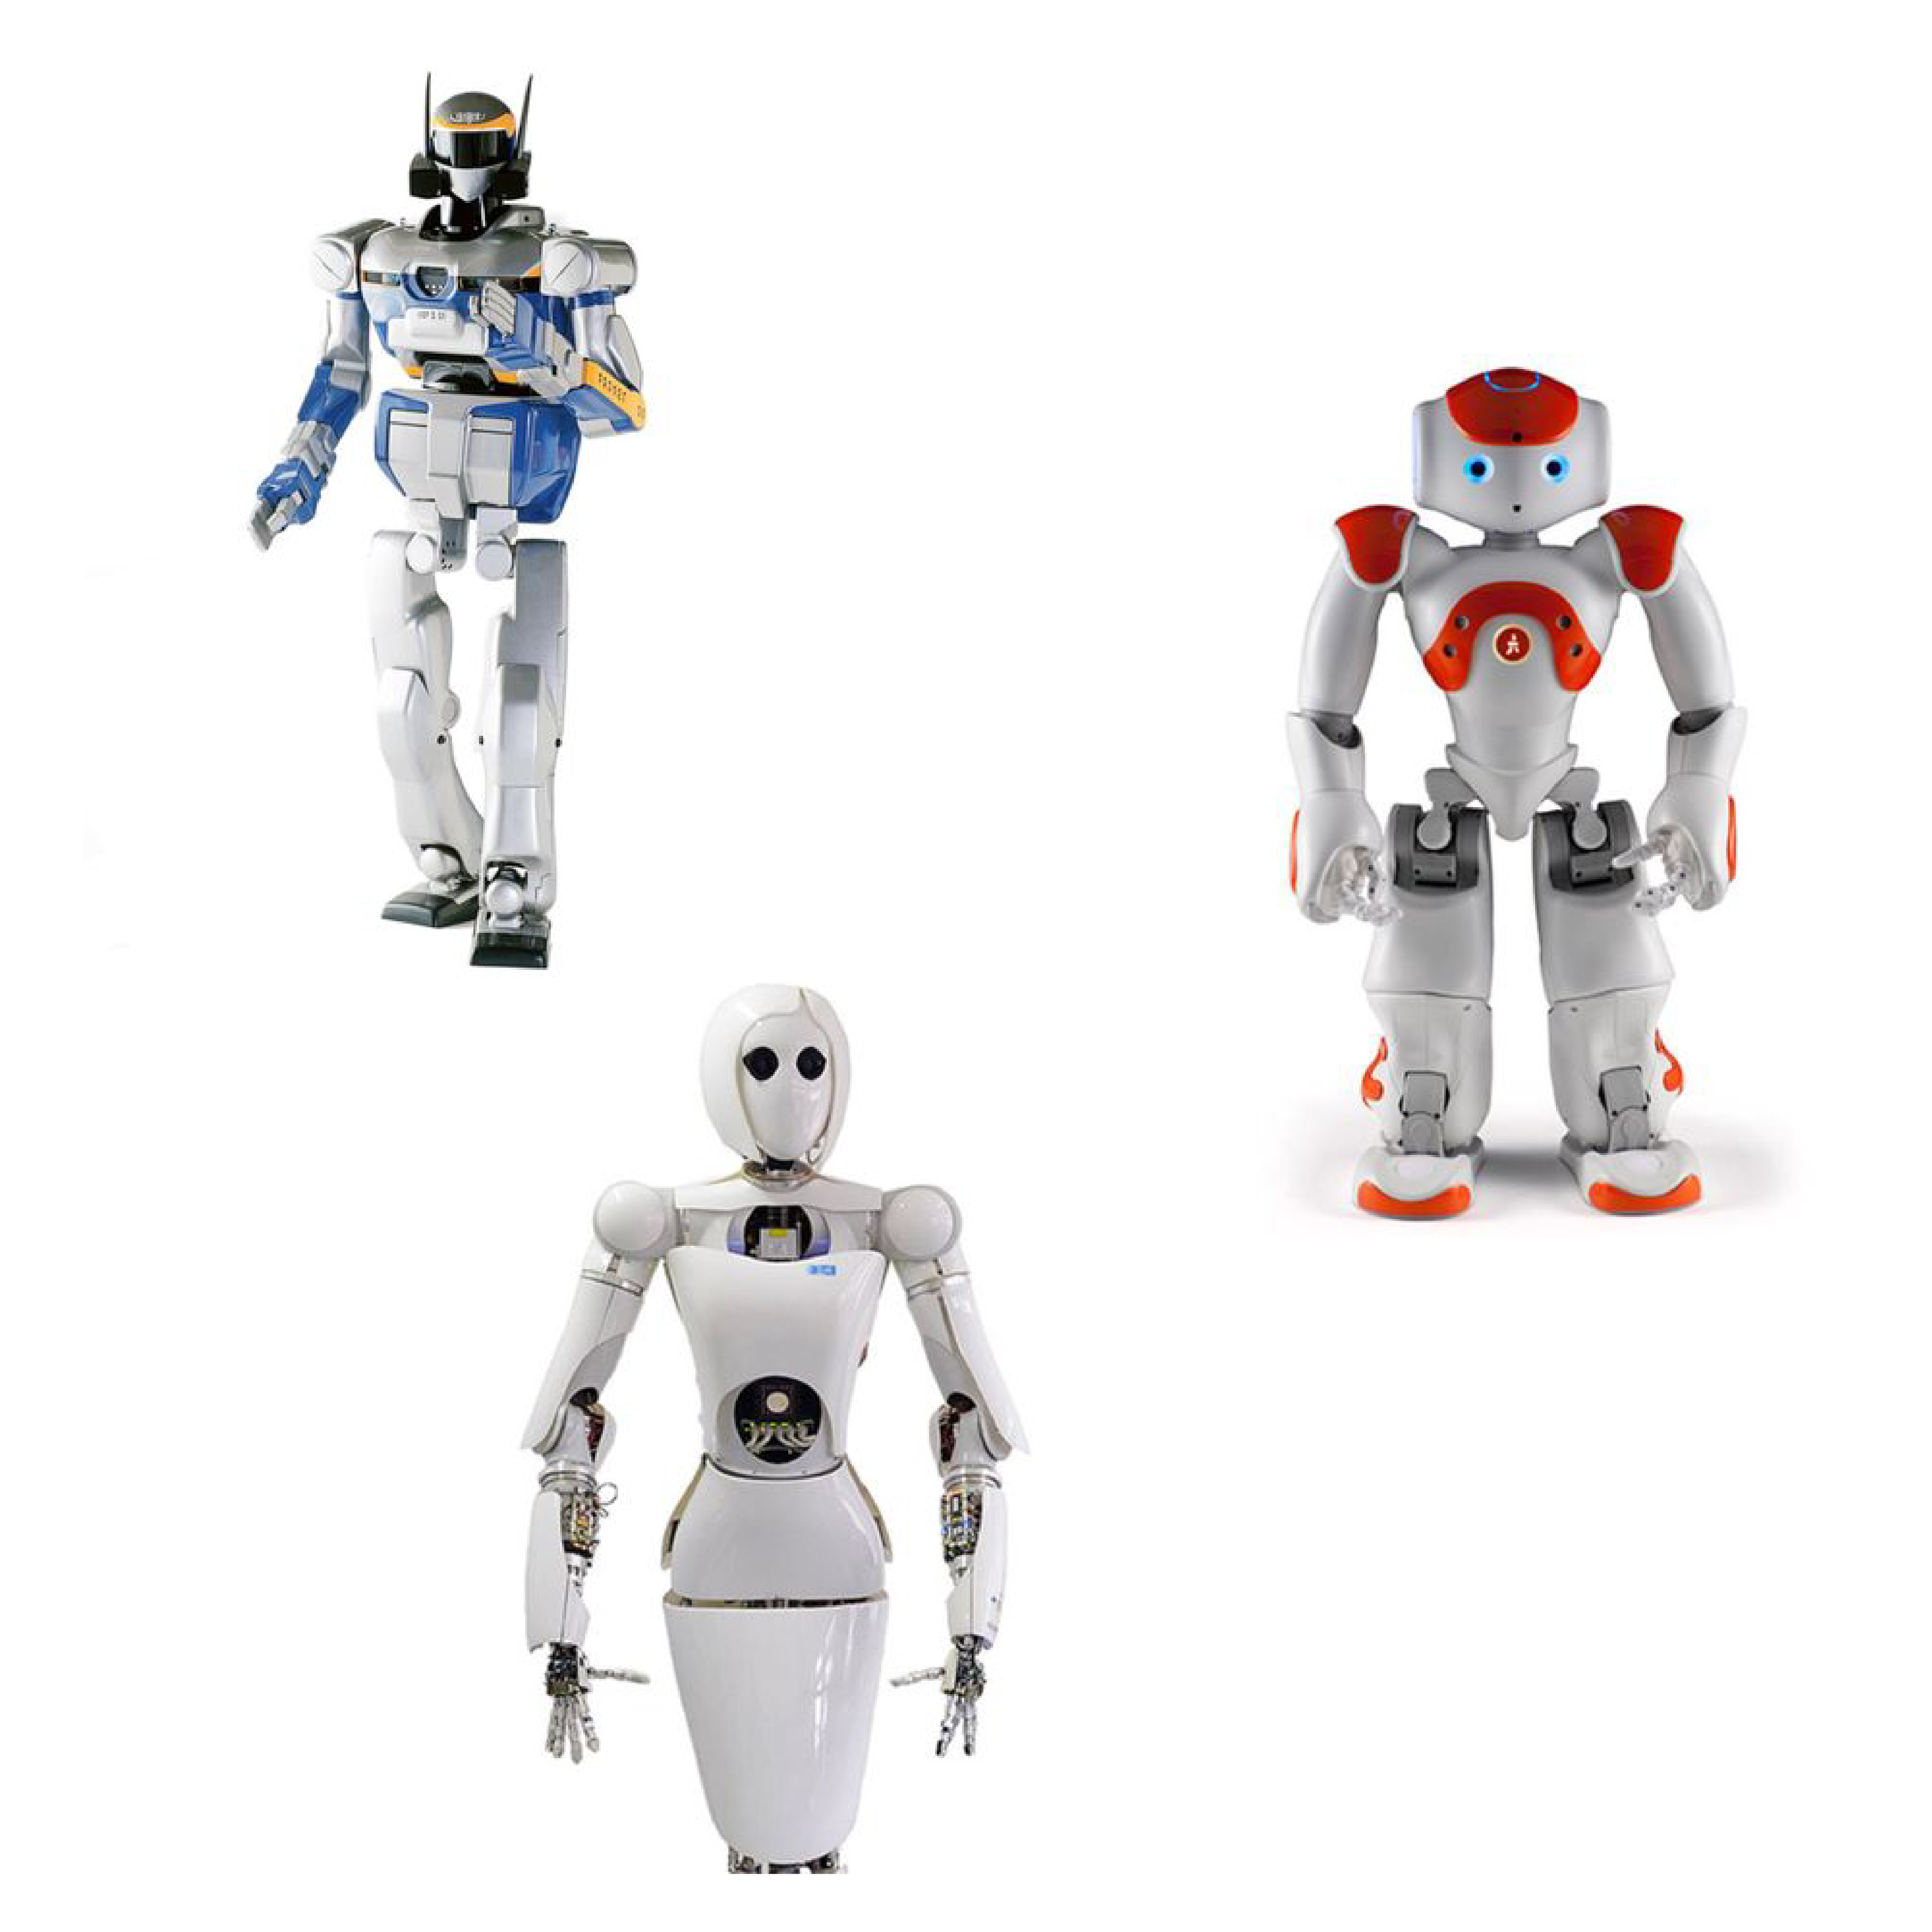
\includegraphics[width=8cm]{images/Humanoid.jpg}}%
          \label{subfig:humanoid}
\subfloat[][機械的ロボット]{%
        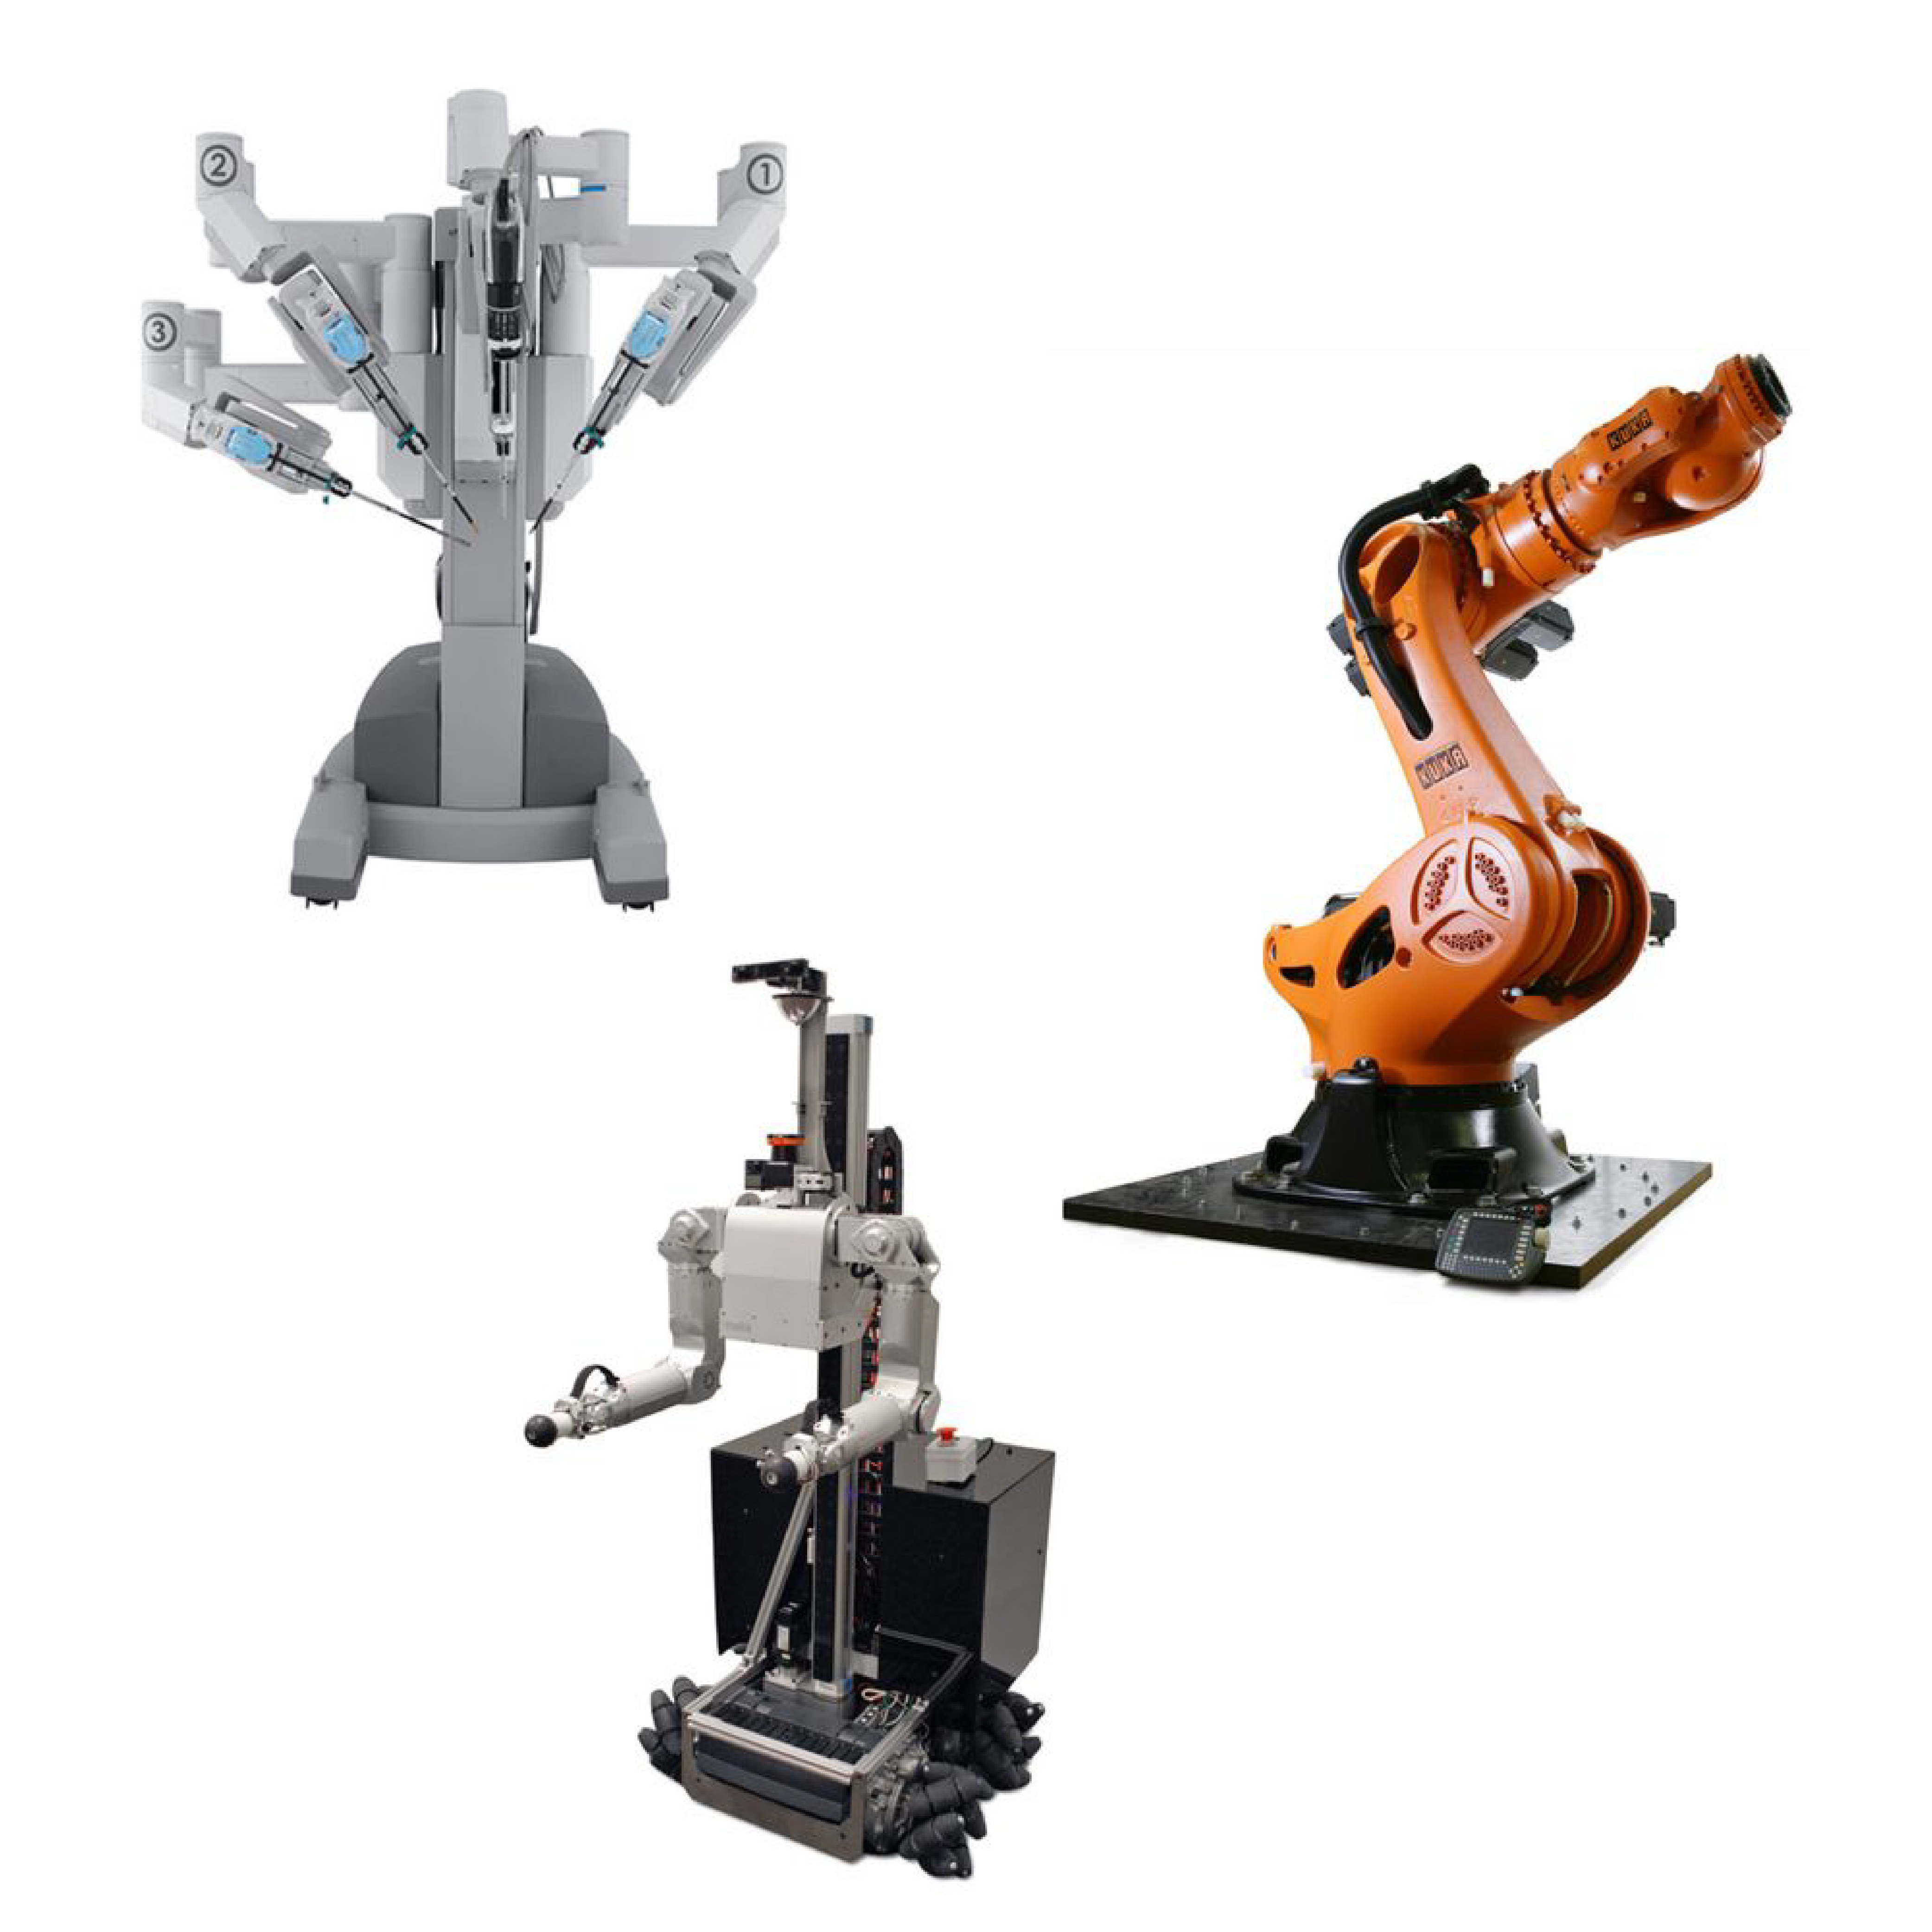
\includegraphics[width=8cm]{images/Mechanoid.jpg}}%
          \label{subfig:machine}
  \caption{質問紙回答時に提示されたロボットの画像}
  \label{fig:Robots}
\end{figure}



\begin{center}
{\scriptsize


%\begin{longtable}{lll}
\begin{longtable}{lp{5cm}p{5cm}}
\caption{質問紙項目}
\label{table:items}
\\\hline
\multicolumn{3}{l}{変数名~~~~~~~~~~~~~~~~~~~~~~~~~~~~~~~~~~~~~~~~~~~~英語  ~~~~~~~~~~~~~~~~~~~~~~~~~~~~~~~~~~~~~~~~~~~~~~~~~~~~~~~~~~~~~~~~~~~~~日本語}\\
\hline \endfirsthead

\\\hline
\multicolumn{3}{l}{変数名~~~~~~~~~~~~~~~~~~~~~~~~~~~~~~~~~~~~~~~~~~~~英語  ~~~~~~~~~~~~~~~~~~~~~~~~~~~~~~~~~~~~~~~~~~~~~~~~~~~~~~~~~~~~~~~~~~~~~日本語}\\
\hline \endhead

\hline
\multicolumn{3}{r}{\scriptsize *反転項目}
\endfoot

ロボットに対する道徳的配慮&A schoolgirl continues to fire a pellet gun at a robot placed in the woods.&ある人が、森に置かれたロボットに向けてエアガンを撃ち続けている\\
&A person making fun robots cleaning dirty drains as they watch.&ある人が、ロボットが汚い排水溝を掃除しているのを見て馬鹿にしている\\
&A person is amused to see a robot being dumped by a person.&ある人が、ロボットが人に捨てられるのを見て面白がっている\\
&A person yells at a robot about how bad the food it made tastes.&ある人が、作った料理の味がひどいとロボットを怒鳴りつけている\\
&A person making fun of a robot for being a bad drawer.&ある人が、絵が下手くそだとロボットを馬鹿にしている\\
&A person threw the robot to the floor because the robot had damaged the furniture.&ある人が、ロボットが家具を傷つけてしまったことを理由にロボットを床に投げ飛ばした\\
&Someone has left a robot outdoors in the rain.&ある人が、ロボットを雨が降っている屋外に放置している\\
&A child is throwing rocks at a robot working on the ranch.&子どもが、牧場で働いているロボットに向かって石を投げつけている\\
&A comedian is jabbing a robot to entertain his audience.&あるコメディアンが、ロボットを叩いて笑いを取ろうとしている\\
&A person beats a robot with a spatula for failing at its job .&ある人が、仕事に失敗したロボットをへらで叩いている\\
&A person is swerving her car in orderto run over a roadside robot.&ある人が、わざと道端のロボットを轢くため車のハンドルを切っている\\
&A person student said that other robots are much more attractive.&ある人が、ロボットに対して他のロボットの方がずっと魅力的だと言っている\\
&A person is telling a robot that it shouldn't be at the entrance because it's too ugly.&ある人がロボットに対して、醜すぎるためエントランスにあるべきではないと言っている\\
宗教への参加&How many times a year do you usually (i.e. before pandemic) visit a religious place (temple, shrine, church etc.)?&コロナウィルス流行以前、あなたは通常年間に約何回ほど宗教施設(寺、神社、教会など)に行っていましたか?\\
宗教的信念&There exists an all-powerful, all-knowing spiritual being, whom we might call Go&霊的で全知全能な神と呼ばれるようなものは実在する。\\
&There exist spiritual beings, who might be good or evil, such as angels or demons.&守護神や悪魔のような善悪のある霊的な存在がいる。\\
&Human beings have immaterial, immortal souls.&人間には、物質的な身体とは区別される魂が存在する。\\
&There is a spiritual realm besides the physical one.&物質的世界以外にも霊的世界が存在する。\\
&There is a spiritual realm besides the physical one.&死後の世界は存在する。\\
&Supernatural events that have no scientific explanation (e.g., miracles) can and do happen.&科学理論では説明できない超自然的な奇跡は起こりうるし、実際に起こる。\\
人間中心主義&The human species is without a doubt the most advanced form of life on earth.&人間は疑うまでもなく地球上で最も進んだ生命体である\\
&Man is the most significant entity in the universe.&人間は地球上で最も重要な種である\\
&If we eventually discover life in other parts of of the universe, such life will probably be found to be inferior to human life.&いずれ我々が宇宙のどこかで生命を見つけたとしても、おそらく人間よりも劣っていると判明するだろう\\
&Humans are superior to all other animals in all important respects.&人間は、すべての重要な性質に関して、他のどの動物よりも優れている\\
&Degree of intelligence ought to be the main measure for determining the superiority of one species over another.&どの生物種が最も優れているかを決める際に、知性を測ることを最重視すべきだ\\
&If there actually is an afterlife, animals are just as likely as humans to take part in such a life after death*.&実際に死後の世界があるとしたら、動物も人間と同じようにその世界に加わるだろう*\\
&Governments should adopt policies which ensure the survival of the human species, even if other species become extinct as a result.&結果的に他の種が絶滅したとしても、政府は人類の生存を確実に保証する政策を採用すべきである\\
&No matter how superiority is defined, it seems that man must be considered superior to all known forms of life.&優越性をどのように定義したとしても、人間は既知のすべての生命体よりも優れている\\
&If I could choose my own afterlife, I would like to be something other than a human being for a change*.&もし生まれ変わって何になるか選べるのなら、私は人間以外の何かになりたい*\\
&Man is the most important species on earth.&人間は宇宙で最も重要な存在である\\
&The primary value of an animal or plant lies in its ability to serve human needs.&動物や植物の最も重要な価値は、人間のニーズ(必要だと思うこと)に応えられることにある\\
アニミズム&I feel that the hand-made object aquires part of the soul of the one that made it.&手作りのモノには作り手の魂の一部が宿っているような気がする\\
&I feel that the mementos have part of the soul of the person who used them.&形見や遺品には、 使っていた人の魂の一部が宿っているような気がする\\
&I feel like my old clothes and old tools have part of the soul of their previous owners.&古着や古道具には以前の所有者の魂の一部が宿っているような気がする\\
&There are times when we feel attachment to things around us like we do to people.&身の回りのモノに、人に対するような愛着を感じることがある\\
&Sometimes I give a human name or pet name to objects around me.&身の回り のモノに人の名前をつけることがある\\
&When I discard something I've used for a long time, I sometimes feel pity for it.&長く愛用していたモノを捨てるときに、 可哀想に思うことがある\\
&I sometimes feel that the things I've used and loved for a long time are another part of myself.&長く愛用しているモノを、自分の分身のように感じることがある\\
&Sometimes I think that the things around me have a human-like mind.&身の回りのモノにも、人間のような心があると思うことがある\\
擬人化傾向&To what extent does technology—devices and machines for manufacturing, entertainment, and productive processes (e.g., cars, computers, television sets)—have intentions?&どの程度、製造・娯楽・生産のための技術的装置と機械(例:自動車・パソコン・テレビ)は意図を持ちますか?\\
&To what extent does the average fish have free will?&どの程度、平均的な魚は自由意志を持ちますか?\\
&To what extent does the average mountain have free will?&どの程度、平均的な山は自由意志を持ちますか?\\
&To what extent does a television set experience emotions?&どの程度、テレビは感情を経験しますか?\\
&To what extent does the average robot have consciousness?&どの程度、平均的なロボットは意識を持ちますか?\\
&To what extent do cows have intentions?&どの程度、牛は意図を持ちますか?\\
&To what extent does a car have free will?&どの程度、自動車は自由意志を持ちますか?\\
&To what extent does the ocean have consciousness?&どの程度、海は意識を持ちますか?\\
&To what extent does the average computer have a mind of its own?&どの程度、平均的なコンピュータはそれ自体が心を持っていますか?\\
&To what extent does a cheetah experience emotions?&どの程度、チーター(ネコ科の動物)は感情を経験しますか?\\
&To what extent does the environment experience emotions?&どの程度、自然環境は感情を経験しますか?\\
&To what extent does the average insect have a mind of its own?&どの程度、平均的な虫はそれ自体に心を持っていますか?\\
&To what extent does a tree have a mind of its own?&どの程度、木はそれ自体に心を持っていますか?\\
&To what extent does the wind have intentions?&どの程度、風は意図を持ちますか?\\
&To what extent does the average reptile have consciousness?&どの程度、平均的な爬虫類は意識を持ちますか?\\
視点取得&Being in a tense emotional situation scares me*.&他の人の視点から物事を見るのは難しいと感じることがある*。\\
&I often have tender, concerned feelings for people less fortunate than me.&何かを決める前には,自分と意見が異なる立場のすべてに目を向けるようにしている。\\
&I would describe myself as a pretty soft-hearted person.&友達のことをよく知ろうとして,その人からどのように物事がみえているか想像する。\\
&I try to look at everybody's side of a disagreement before I make a decision*.&自分が正しいと思える時には,他の人の言い分を聞くようなことには時間を使わない*。\\
&If I'm sure I'm right about something, I don't waste much time listening to other people's arguments.&すべての問題点には2つの立場があると思っており,その両者に目を向けるようにしている\\
&When I watch a good movie, I can very easily put myself in the place of a leading character&誰かにいらいらしているときにはたいてい,しばらくその人の身になって考えるようにしている。\\
&Becoming extremely involved in a good book or movie is somewhat rare for me.&誰かを批判する前には,自分が批判される相手の立場だったらどう感じるか想像しようとする。\\
共感的関心&I sometimes feel helpless when I am in the middle of a very emotional situation.&自分より不運な人たちを心配し,気にかけることが多い。\\
&I tend to lose control during emergencies*.&他の人たちが困っているのを見て,気の毒に思わないことがある*。\\
&When I see someone being taken advantage of, I feel kind of protective towards them.&誰かがいいように利用されているのをみると,その人を守ってあげたいような気持ちになる。\\
&When I see someone being treated unfairly, I sometimes don't feel very much pity for them*.&他の人たちが不運な目にあっているのはたいてい,それほど気にならない*。\\
&When I'm upset at someone, I usually try to ``put myself in his shoes'' for a while*.&誰かが不公平な扱いをされているのをみたときに,そんなにかわいそうだと思わないことがある*。\\
&I sometimes find it difficult to see things from the ``other guy's'' point of view.&自分が見聞きした出来事に,心を強く動かされることが多い。\\
&I daydream and fantasize, with some regularity, about things that might happen to me.&自分は思いやりの気持ちが強い人だと思う。\\
ロボット関連メディア接触&How often do you watch robot-related media contents? (e.g., stories, comics, news articles, academic articles, animes, video games, television, DVD, internets)&どれぐらいロボットに関連したメディアを見ますか?(例:小説、漫画、ニュース記事、論文、アニメ、テレビゲーム、テレビ、DVD、インターネット)\\
&How often do you touch robots directly?&直接ロボットに触る機会はどれくらいありますか?\\
&How often do you build or program robot?&自分でロボットのプログラミングをしたり、作ったりする機会はどれくらいありますか?\\
典型的ロボットイメージ&Which of the following images, A or B, is closer to your image of a robot?&以下に示すA、Bのうち、どちらがあなたが考えるロボットのイメージに近いですか?



\end{longtable}
}

\end{center}






\subsection{分析方法}
\subsubsection{仮説H1の検証}
H1「日本のほうがアメリカよりロボットに対する道徳的配慮が高い」を検証するために、二国間の参加者のロボットに対する道徳的配慮尺度の点数の平均値を比較した。対応のない$t$検定による平均値の差の有意性の検証を行い、さらに効果量の検討を行った。

\subsubsection{仮説H2の検証}
H2「日本では、宗教性が高い人ほどロボットに対する道徳的配慮が高い。逆にアメリカでは、宗教性が高い人ほどロボットに対する道徳的配慮が低い」を検証するために、宗教性を説明変数とした重回帰分析を行った。仮説検証の手順は以下2つのモデルを比較することで行った。第一のモデル (model 1a) では、国籍と宗教性 (宗教への参加、宗教的信念) を説明変数とした回帰を行う。第二のモデル (model 1b) では、国籍と宗教性、国籍×宗教性の交互作用を説明変数とした回帰を行う。回帰分析においては、年齢、性別、教育歴、PT、EC、ロボット関連メディア接触、典型的ロボットイメージ、およびそれらと国籍 (2値変数で、日本を0、アメリカを1とした) の交互作用を統制変数として投入した。また、2値変数以外の変数は標準化を行った。



もし、model 1aに比べmodel 1bの当てはまりおよび予測力が高く、日本で正、アメリカで負の効果を示す国籍×宗教性の交互作用が存在すれば (日本を1、アメリカを0としているため、負の主効果が存在し、かつそれを上回る大きさの正の交互作用の認められた場合に仮説と一致したとみなされる) 、仮説が支持されたと判断することとした。また、国籍を考慮しないモデル (null model) を実行し、ベースラインを示した。当てはまりの比較は残差の差の検定、予測力の比較はAkaike's Information Criterion (AIC) 基準を用いて行った。それぞれの変数の影響は有意水準を$\alpha=0.05$として有意性を判断した。



ただし、宗教については2種類の変数を測定したため、その扱いについてはデータを確認した後に決定した。事前に以下の手続きを行うことを決定していた。宗教への参加と宗教的信念の間に高い一貫性があれば、それらを合成変数として扱い、そうでない場合には別の変数として扱う。後者の場合には、2つの変数が目的変数に与える影響がどのように違い、それがどのような要因によるのかを考察する。

\subsubsection{仮説H3、4の検証}
H3「日本では、宗教性がアニミズムに正、人間中心主義に負の影響を持つ。逆にアメリカでは、宗教性が人間中心主義に正、アニミズムに負の影響を持つ」、H4「どちらの国でも、ロボットに対する道徳的配慮に対して、アニミズムが正の、人間中心主義が負の影響を持つ」を検証するため、上記の仮説を表したパスモデルへの当てはめを行った。モデルへの当てはめは、共分散構造分析の多母集団同時解析 (multi-group SEM) によって行った。同時解析によって、検定の繰り返しによる第一種の過誤のリスクを抑えることができる。潜在変数間のパスの大きさを効果量として比較するため、潜在変数の分散は1に固定した。この解析では、ジェンダーをその他と回答した参加者を除いて解析を行った。理由は、該当する参加者が少なく (日本で0.7\%、アメリカで0.3\%) 解釈可能な結果を得ることが難しいと判断したからである。


モデルの当てはめは、最尤法によって行った。SEMの当てはめによる仮説検証を行っている先行研究\cite{noren}にならい、当てはまりの評価はRMSEA (Root Mean Square Error of Approximation) とCFI (Comparative Fit Index) によって行った。また、GFI( Goodness-of-Fit Index) およびAGFI (Adjusted Goodness-of-Fit Index) も補助的に検討した。
CFIおよびRMSEAは尤度比検定統計量の非心性 (noncentrality) を利用した指標である\cite{hishin} 。最も制約がない、すなわち構造を考慮しないモデル (飽和モデル) と仮説モデルの間の尤度比検定統計量を$T_h$とすると、$T_h$は仮説モデルが正しい場合には自由度$df$の$\chi^2$分布 (非心度 $\lambda$: noncentrality parameter が0) に漸近的に従う。ここで$df$とは仮説モデルに課されている制約の数である。飽和モデルが正しい場合には、自由度$df$の非心$\chi^2$分布に漸近的に従う。このとき、非心度を$\lambda_h$と表した場合$\lambda_h=T_h - df$であるが、この値は0に近ければ仮説モデルがより良いモデルであるとみなせる。CFIは、$\lambda_h$をベースラインモデル (すべての変数間を独立であるとみなしたモデル) の非心度$\lambda_b$で規格化されており、仮説モデルが飽和モデルと同じ当てはまりを持つ場合に1に、ベースラインモデルと同じ当てはまりを持つ場合に0になる。経験的には、CFIは0.95を超えると当てはまりが良いとみなされる。RMSEAは非心度をサンプル数の自由度で割ったものを$df$で割ったものであり、制約あたりの非心度と考えることができる。この値は経験的に、0.05を下回ると当てはまりが良いとみなされる。GFI、AGFIはデータの共分散行列と、モデルによって説明される共分散行列の乖離を表す指標である\cite{hishin} 。AGFIはGFIを観測変数およびモデルの自由度で補正した指標であり、GFI$>=$AGFIである。両者とも0から1までの値を取り、0.95を超えると当てはまりが良いとみなされる。
$\chi ^2$統計量による検定を用いれば、「データが持つ構造と仮説の構造が同じ」という帰無仮説が棄却されるかどうかを検証することが可能である (棄却されない場合、仮説の構造がデータの分散を良く説明するとみなすことができる) が、本研究では実験参加者数が多いことから、過剰に保守的な検定となってしまう。そのため$\chi ^2$統計量による検定は実施しなかった。この手法も、先行研究\cite{noren}にならったものである。
% 構造方程式モデリングにおける適合度指標とモデル改善について

以上の基準によりモデルの適合度を評価した後、仮説モデルが採択可能なモデルであった場合にはパス係数を評価し、仮説検証を行った。
具体的には、以下の4つの予測を検証した。
\begin{description}
\item{H3} 日本では、宗教性がアニミズムに正、人間中心主義に負の影響を持つ。逆にアメリカでは、宗教性が人間中心主義に正、アニミズムに負の影響を持つ。
\begin{description}
\item{i) } 宗教性は、日本ではアニミズムに正、アメリカではアニミズムに負のパス
\item{ii)} 宗教性は、日本では人間中心主義に負、アメリカでは人間中心主義に正のパス
\end{description}


\item{H4} どちらの国でも、ロボットに対する道徳的配慮に対して、アニミズムが正の、人間中心主義が負の影響を持つ。
\begin{description}
\item{iii)} 両方の国でアニミズムからロボットに対する道徳的配慮に正のパス
\item{iv)} 両方の国で人間中心主義からロボットに対する道徳的配慮に負のパス
\end{description}
\end{description}

パス係数の評価に加え、二国間でのパス係数の差を探索的に分析した。そのために、 a) 注目しているパスを二国間で固定したモデルと b) すべてのパスが二国間で異なるようにしたモデルを尤度の差によって比較した。モデル b) の当てはまりが a) よりも有意によければ (すなわち注目しているパスの係数を二国間で違えたほうが当てはまりがよければ) 、注目しているパスは二国間で有意に異なると判断した。


以上の分析は、R 4.0.3 および、lavaan 0.6-7パッケージ\cite{lavaan}.を用いて行った。

\section{結果}
\subsection{仮説H1:ロボットに対する道徳的配慮に文化差はあるか?}
測定した変数の記述統計量およびそれらの相関行列は表\ref{tab:Table_Desc}と表\ref{tab:Table_Cor_JP}、表\ref{tab:Table_Cor_US}に示した。ロボットに対する道徳的配慮は日本のほうが有意に高く ($t(3108.2) = -16.3, p = .000$) 、これは仮説H1と一致する。効果量は中程度 ($|d| = 0.54$) であった。今回使用したMoral care for robots scaleは、ロボットを物理的に攻撃する内容だけでなく (例:ある人が、ロボットが家具を傷つけてしまったことを理由にロボットを床に投げ飛ばした。) ロボットの名誉を傷つける内容 (例:ある人が、ロボットに対して新しいロボットの方がずっと魅力的だと言っている。) も含まれていた。そして、尺度の一貫性は非常に高かった (日本で$\alpha=.95$、アメリカで$\alpha=.96$) 。以上のことから、例えばロボットが高価であるから傷つけてはいけない、といった理由ではなく (この可能性は、先行研究\cite{okanda}で用いられた尺度では排除できていなかった) 、ロボットが物理的あるいは社会的に攻撃されることを嫌う度合いが測定されていたと判断できる。

\begin{landscape}
\begin{table}[h]
  \begin{threeparttable}
\caption{即位変数の平均と標準偏差および文化間の差異}
\label{tab:Table_Desc}
\begin{tabular}{@{}llllllllll@{}}
\toprule
\multirow{2}{*}{測定変数}          &           & \multicolumn{2}{l}{アメリカ} &  & \multicolumn{2}{l}{日本} &  & \multicolumn{2}{l}{差異} \\ \cmidrule(lr){3-4} \cmidrule(lr){6-7} \cmidrule(l){9-10} 
                                  & Scale     & Mean          & SD            &  & Mean            & SD             &  & Cohen's $d$ & 95\% CI            \\ \midrule
ロボットへの道徳的配慮 & (1 to 7)  & 4.73          & 1.71          &  & 5.51            & 1.15           &  & -0.54     & {[}-0.61, -0.47{]} \\
宗教への参加                 & (0 to 10) & 4.96          & 4.15          &  & 2.28            & 2.85           &  & 0.76      & {[}~0.69, ~0.82{]}   \\
宗教的信念                & (-4 to 4) & 2.37          & 1.82          &  & 0.39            & 1.90           &  & 1.07      & {[}~1.00, ~1.13{]}   \\
人間中心主義                  & (1 to 7)  & 4.27          & 1.26          &  & 3.88            & 1.00           &  & 0.39      & {[}~0.28, ~0.41{]}   \\
アニミズム                           & (1 to 5)  & 3.39          & 0.96          &  & 3.38            & 0.80           &  & 0.02      & {[}-0.05, ~0.08{]}  \\
擬人化傾向                  & (0 to 10) & 4.76          & 2.36          &  & 4.82            & 1.75           &  & -0.03     & {[}-0.09, ~0.04{]}  \\
視点取得              & (1 to 7)  & 5.04          & 0.99          &  & 4.19            & 0.82           &  & 0.93      & {[}~0.86, ~1.00{]}   \\
共感的関心          & (1 to 7)  & 5.29          & 1.10          &  & 4.61            & 0.95           &  & 0.67     & {[}~0.60, ~0.73{]}   \\
典型的ロボットイメージ *  & (0 to 1)  & 0.17          & 0.38          &  & 0.24            & 0.43           &  &      &   \\ 
ロボット関連メディア接触   & (1 to 8)  & 3.10          & 1.86          &  & 3.09            & 1.40           &  & 0.01      & {[}-0.06, ~0.07{]}  \\\bottomrule
\end{tabular}
\begin{tablenotes}
      \small
      \item $^{*}$0:ヒューマノイドロボット、1:機械的ロボット
 \end{tablenotes}
  \end{threeparttable}

\end{table}
\end{landscape}


\begin{table}[H]
{\scriptsize
  \begin{threeparttable}
\caption{日本のサンプルにおける相関行列 (Spearman's $\rho$) }
\label{tab:Table_Cor_JP}
\begin{tabular}{@{}lllllllllllllll@{}}
\toprule
     & MR & RA    & SBS        & ACE        & ANI        & AM         & PT         & EC         & TYP   & EXP        & Age        & Edu        & Gen1       & Gen2        \\ \midrule
MR   &    & -0.04 & ~0.19 & -0.01      & ~0.23 & ~0.22 & ~0.16 & ~0.29 & 0.09  & -0.04      & -0.05      & -0.11      & ~0.24 & ~0.01  \\
RA   &    &       & ~0.15 & -0.03      & ~0.16 & ~0.09 & ~0.11 & ~0.12 & -0.11 & ~0.27 & ~0.10 & ~0.12 & -0.03      & ~0.01  \\
SBS  &    &       &            & ~0.05 & ~0.41 & ~0.47 & ~0.22 & ~0.29 & 0.07  & ~0.13 & -0.05      & -0.05      & ~0.08 & ~0.02  \\
ACE  &    &       &            &            & ~0.08 & ~0.04 & ~0.08 & ~0.04 & 0.09  & ~0.05 & -0.03      & -0.05      & -0.02      & -0.05 \\
ANI  &    &       &            &            &            & ~0.38 & ~0.31 & ~0.03 & 0.04  & ~0.22 & -0.11      & ~0.06 & ~0.11 & ~0.01  \\
AM   &    &       &            &            &            &            & ~0.24 & ~0.20 & 0.02  & ~0.16 & -0.06      & -0.03      & ~0.01 & ~0.02  \\
PT   &    &       &            &            &            &            &            & ~0.49 & -0.03 & ~0.20 & -0.01      & ~0.07 & ~0.04 & ~0.03  \\
EC   &    &       &            &            &            &            &            &            & 0.02  & ~0.12 & ~0.00 & -0.03      & ~0.12 & ~0.00  \\
TYP  &    &       &            &            &            &            &            &            &       & -0.06      & -0.09      & -0.03      & ~0.08 & ~0.01  \\
EXP  &    &       &            &            &            &            &            &            &       &            & -0.06      & ~0.12 & -0.09      & ~0.00  \\
Age  &    &       &            &            &            &            &            &            &       &            &            & ~0.06 & -0.37      & -0.02       \\
Edu  &    &       &            &            &            &            &            &            &       &            &            &            & -0.10      & -0.01       \\
Gen1 &    &       &            &            &            &            &            &            &       &            &            &            &            & -0.09       
\\ \bottomrule
\end{tabular}
  \begin{tablenotes}
      \small
      \item ~~
    \end{tablenotes}
  \end{threeparttable}
  }
\end{table}

\begin{table}[H]
{\scriptsize
  \begin{threeparttable}
\caption{アメリカのサンプルにおける相関行列 (Spearman's $\rho$) }
\label{tab:Table_Cor_US}
\begin{tabular}{@{}lllllllllllllll@{}}
\toprule
     & MR & RA    & SBS        & ACE        & ANI        & AM         & PT         & EC         & TYP        & EXP        & Age        & Edu        & Gen1       & Gen2       \\ \midrule
MR   &    & -0.11 & ~0.00 & -0.33      & -0.11      & -0.19      & ~0.21 & ~0.39 & -0.08      & -0.26      & ~0.02 & -0.19      & ~0.28 & ~0.02 \\
RA   &    &       & ~0.43 & ~0.34 & ~0.12 & ~0.11 & ~0.10 & ~0.09 & ~0.07 & ~0.30 & ~0.07 & ~0.33 & -0.17      & -0.03      \\
SBS  &    &       &            & ~0.29 & ~0.19 & ~0.08 & ~0.26 & ~0.27 & ~0.02 & ~0.10 & ~0.09 & ~0.04 & -0.01      & -0.03      \\
ACE  &    &       &            &            & ~0.25 & ~0.16 & ~0.00 & -0.10      & ~0.20 & ~0.24 & ~0.09 & ~0.25 & -0.25      & -0.07      \\
ANI  &    &       &            &            &            & ~0.51 & ~0.12 & -0.02      & ~0.09 & ~0.32 & -0.14      & ~0.18 & ~0.00 & -0.01      \\
AM   &    &       &            &            &            &            & ~0.02 & -0.16      & ~0.06 & ~0.36 & -0.14      & ~0.21 & -0.08      & ~0.03 \\
PT   &    &       &            &            &            &            &            & ~0.59 & -0.05      & ~0.04 & ~0.04 & ~0.00 & ~0.07 & -0.03      \\
EC   &    &       &            &            &            &            &            &            & -0.06      & -0.14      & ~0.10 & -0.12      & ~0.19 & ~0.02 \\
TYP  &    &       &            &            &            &            &            &            &            & ~0.01 & -0.06      & ~0.10 & ~0.00 & -0.03      \\
EXP  &    &       &            &            &            &            &            &            &            &            & -0.02      & ~0.35 & -0.32      & -0.01      \\
Age  &    &       &            &            &            &            &            &            &            &            &            & ~0.08 & -0.16      & -0.04      \\
Edu  &    &       &            &            &            &            &            &            &            &            &            &            & -0.27      & -0.03      \\
Gen1 &    &       &            &            &            &            &            &            &            &            &            &            &            & -0.06      \\
 \bottomrule
\end{tabular}
    \begin{tablenotes}
      \small
      \item MR:ロボットに対する道徳的配慮、RA:宗教への参加、SBS:宗教的信念、ACE:人間中心主義、ANI:アニミズム、AM:擬人化傾向、PT:視点取得、EC:共感的関心、TYP:典型的ロボットイメージ、EXP:ロボット関連メディア接触、Gen1:女性、Gen2:その他
    \end{tablenotes}
  \end{threeparttable}
  }
\end{table}







\subsection{宗教性の測定結果}
測定した2種類の宗教性 (宗教への参加、宗教的信念) の間の一貫性は、とくに日本においては低かった。このことから、これらを別の変数として扱った。以下の分析では、それぞれの変数の影響を個別に検証し考察した。


宗教への参加と宗教的信念の相関 (Spearman's correlation) は、日本で$\rho=.15$、アメリカで$\rho=.43$であり、多重共線性が生じる可能性は無視できる。
それぞれの変数の分布は図\ref{fig:Figure_Inte}に示した。
\begin{figure}[H]
  \centering
  
\subfloat[][日本における宗教への参加]{%
        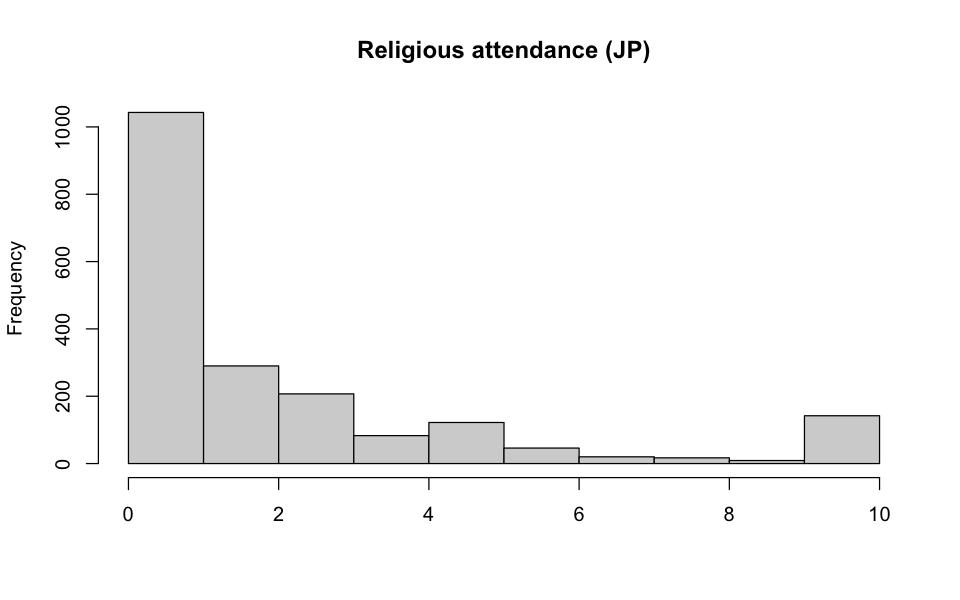
\includegraphics[width=8cm]{images/relatt_jp.png}}%
\subfloat[][アメリカにおける宗教への参加]{%
        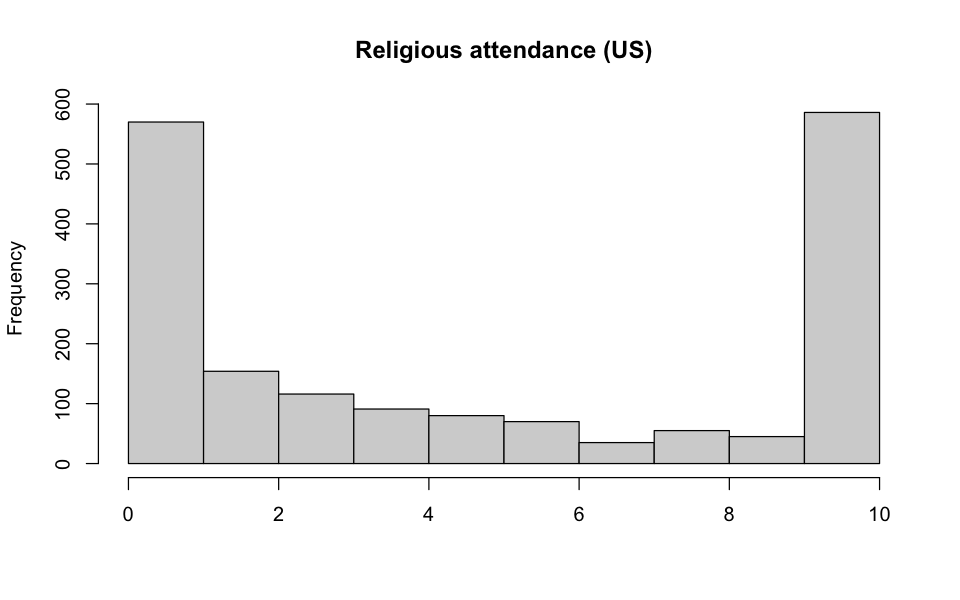
\includegraphics[width=8cm]{images/relatt_us.png}}%
  
\subfloat[][日本における宗教的信念]{%
        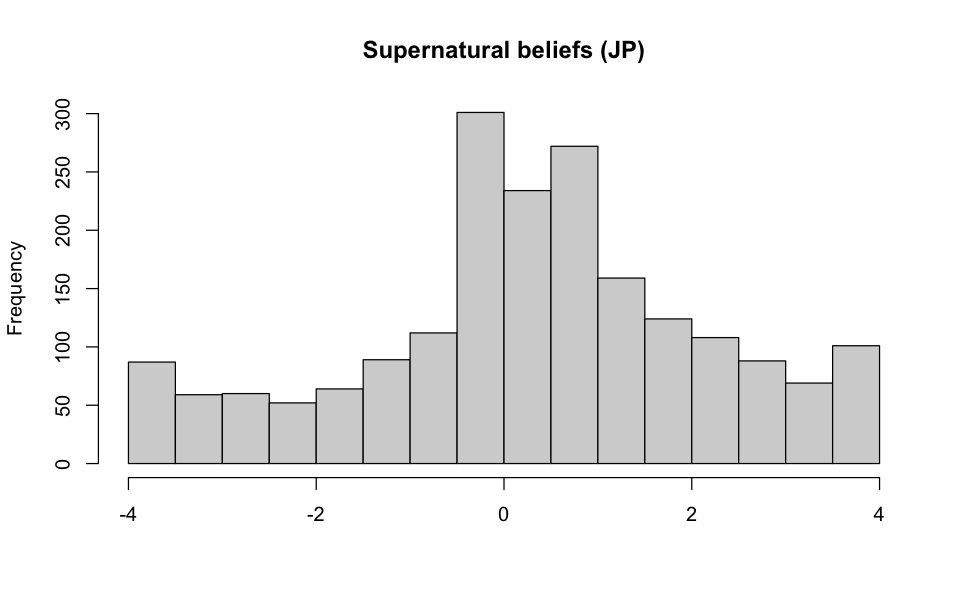
\includegraphics[width=8cm]{images/sbs_jp.png}}%  
\subfloat[][アメリカにおける宗教的信念]{%
        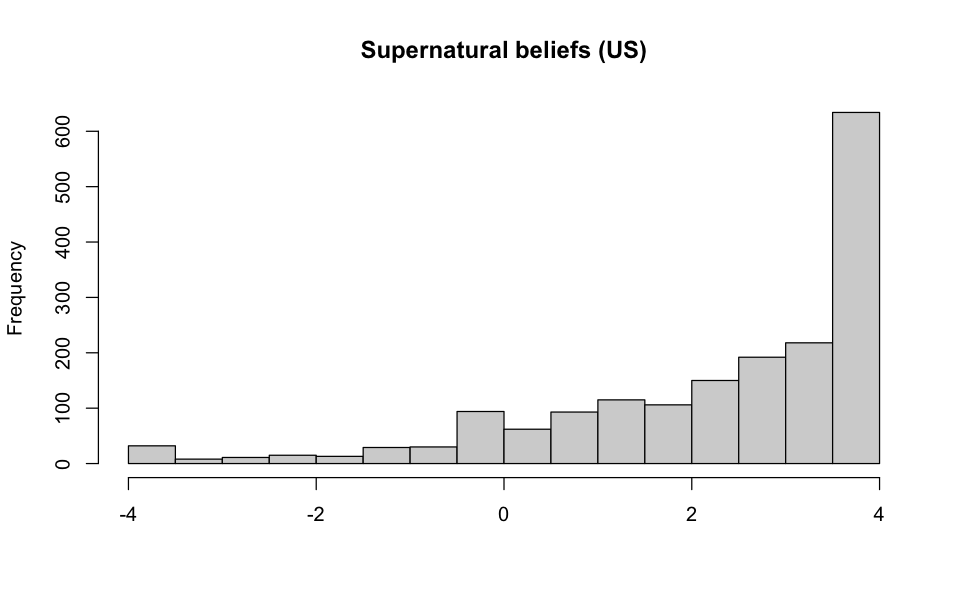
\includegraphics[width=8cm]{images/sbs_us.png}}%
  \caption[宗教への参加および宗教的信念の得点の分布]{宗教への参加および宗教的信念の得点の分布。ただし、宗教への参加の数値化は1 (0回) 、2 (1回) 、3 (2回) 、4 (3回) 、5 (4回) 、6 (5回) 、7 (6回) 、8 (7回) 、9 (8回) 、10 (9回) 、11 (10回以上) として行った。}
  \label{fig:Figure_Inte}
\end{figure}















\subsection{仮説H2:宗教の影響は文化間でどのように違うのか?}
仮説H2の検証は、ロボットに対する道徳的配慮を目的変数とした回帰分析において、国籍と宗教性の交互作用を考慮しないモデル (model 1a) と考慮するモデル (model 1b) を残差およびAICの差を検討することによって実施した。


回帰分析の結果を表\ref{tab:Table_Regr}に示した。残差の検定の結果、model 1bがよりよく当てはまっていることが示された ($\Delta deviance = 8.33, p = .016$) 。また、AIC基準による比較でも、model 1bがよい予測力を持つことが示された。


\clearpage
\begin{table}[]
{\scriptsize
  \begin{threeparttable}
\caption{仮説H2の検証のための回帰分析}
\label{tab:Table_Regr}
\begin{tabular}{@{}lllllllll@{}}
\toprule
\multirow{2}{*}{説明変数}                & \multicolumn{2}{l}{null model}        &  & \multicolumn{2}{l}{model 1a}          &  & \multicolumn{2}{l}{model 1b}          \\ \cmidrule(lr){2-3} \cmidrule(lr){5-6} \cmidrule(l){8-9} 
                                          & β              & 95\%CI               &  & β              & 95\%CI               &  & β              & 95\%CI               \\ \midrule
切片                                 & -0.13$^*$  & {[}-0.05, -0.21{]}   &  & ~0.10         & {[}~0.22, -0.01{]}  &  & ~0.13$^*$ & {[}~0.25, ~0.02{]} \\
仮説に関連する説明変数                    &                &                      &  &                &                      &  &                &                      \\
~~宗教への参加 (RA)             & -0.11$^{***}$       & {[}-0.07, -0.14{]}   &  & -0.03          & {[}~0.00, -0.06{]}  &  & -0.02          & {[}~0.03, -0.07{]}  \\
~~宗教的信念 (SBS)            & -0.12$^{***}$       & {[}-0.09, -0.16{]}   &  & -0.04$^*$  & {[}~0.00, -0.08{]}  &  & ~0.01         & {[}~0.06, -0.04{]}  \\
~~国籍 (CC)           &                &                      &  & -0.51$^{***}$       & {[}-0.35, -0.66{]}   &  & -0.51$^{***}$       & {[}-0.36, -0.67{]}   \\
仮説に関連する説明変数   (交互作用)    &                &                      &  &                &                      &  &                &                      \\
~~宗教への参加×国籍                                 &                &                      &  &                &                      &  & ~0.00         & {[}~0.07, -0.07{]}  \\
~~宗教的信念×国籍                         &                &                      &  &                &                      &  & -0.10$^*$  & {[}-0.03, -0.18{]}   \\
共変量                               &                &                      &  &                &                      &  &                &                      \\
~~擬人化傾向                & ~0.00         & {[}~0.03, -0.03{]}  &  & ~0.15$^{***}$      & {[}~0.20, ~0.10{]} &  & ~0.13$^{***}$      & {[}~0.18, ~0.08{]} \\
~~視点取得               & -0.07$^{***}$       & {[}-0.03, -0.11{]}   &  & ~0.00         & {[}~0.06, -0.06{]}  &  & ~0.00         & {[}~0.05, -0.06{]}  \\
~~共感的関心                & ~0.29$^{***}$      & {[}~0.33, ~0.25{]} &  & ~0.22$^{***}$      & {[}~0.27, ~0.17{]} &  & ~0.21$^{***}$      & {[}~0.27, ~0.16{]} \\
~~典型的ロボットイメージ                   & ~0.03         & {[}~0.11, -0.04{]}  &  & ~0.11$^*$ & {[}~0.21, ~0.01{]} &  & ~0.11$^*$ & {[}~0.21, ~0.01{]} \\
~~ロボット関連メディア接触 & -0.12$^{***}$       & {[}-0.09, -0.15{]}   &  & -0.06$^*$  & {[}-0.02, -0.11{]}   &  & -0.07$^*$  & {[}-0.02, -0.12{]}   \\
~~年齢                                  & ~0.05$^*$ & {[}~0.08, ~0.02{]} &  & ~0.04         & {[}~0.08, ~0.00{]} &  & ~0.04         & {[}~0.08, ~0.00{]} \\
~~教育歴                             & -0.14$^{***}$       & {[}-0.08, -0.20{]}   &  & -0.12$^*$  & {[}-0.04, -0.20{]}   &  & -0.12$^*$  & {[}-0.04, -0.19{]}   \\
~~ジェンダー1                               & ~0.34$^{***}$      & {[}~0.41, ~0.28{]} &  & ~0.28$^{***}$      & {[}~0.37, ~0.20{]} &  & ~0.28$^{***}$      & {[}~0.37, ~0.20{]} \\
~~ジェンダー2                               & ~0.45$^*$ & {[}~0.85, ~0.04{]} &  & ~0.26         & {[}~0.71, -0.19{]}  &  & ~0.25         & {[}~0.71, -0.20{]}  \\
共変量  (交互作用)                  &                &                      &  &                &                      &  &                &                      \\
~~擬人化傾向×国籍                               &                &                      &  & -0.30$^{***}$       & {[}-0.23, -0.36{]}   &  & -0.27$^{***}$       & {[}-0.20, -0.33{]}   \\
~~視点取得×国籍                                &                &                      &  & ~0.02         & {[}~0.10, -0.06{]}  &  & ~0.02         & {[}~0.10, -0.05{]}  \\
~~共感的関心×国籍                                 &                &                      &  & ~0.08$^*$ & {[}~0.15, ~0.01{]} &  & ~0.10$^*$ & {[}~0.17, ~0.03{]} \\
~~典型的ロボットイメージ×国籍                                 &                &                      &  & -0.22$^*$  & {[}-0.08, -0.35{]}   &  & -0.21$^*$  & {[}-0.07, -0.34{]}   \\
~~メディア接触×国籍                                &                &                      &  & -0.11$^{***}$       & {[}-0.04, -0.17{]}   &  & -0.10$^*$  & {[}-0.04, -0.17{]}   \\
~~年齢×国籍                                &                &                      &  & -0.04          & {[}~0.01, -0.10{]}  &  & -0.04          & {[}~0.02, -0.10{]}  \\
~~教育歴×国籍                          &                &                      &  & ~0.04         & {[}~0.16, -0.07{]}  &  & ~0.03         & {[}~0.15, -0.08{]}  \\
~~ジェンダー1×国籍                            &                &                      &  & ~0.04         & {[}~0.16, -0.08{]}  &  & ~0.05         & {[}~0.17, -0.07{]}  \\
~~ジェンダー2×国籍                            &                &                      &  & ~0.23         & {[}~1.06, -0.59{]}  &  & ~0.23         & {[}~1.05, -0.60{]}  \\
                                          &                &                      &  &                &                      &  &                &                      \\
                                          &                &                      &  &                &                      &  &                &                      \\
$R^2$ Adj.                                & 0.170          &                      &  & 0.270          &                      &  & 0.273          &                      \\
AIC                                       & 10039.4        &                      &  & 9557.4         &                      &  & 9553.1         &                      \\
$Log$ Lik.                                & -5006.7        &                      &  & -4755.7        &                      &  & -4751.6        &                      \\ \bottomrule
\end{tabular}
    \begin{tablenotes}
      \small
      \item $^{1}$ カテゴリカル変数以外の変数はサンプル全体の平均と標準偏差を用いた標準化を行った。 カテゴリカル変数は2値のダミー変数でコーディングした。具体的には、ジェンダー (男性:ジェンダー1 = 0、ジェンダー2 = 0;女性:ジェンダー1 = 0、ジェンダー2 = 1;その他:ジェンダー1 = 0、ジェンダー2 = 1)、国籍 (日本:0;アメリカ:1)、教育歴 (大卒より長い教育歴:1、それ以外:0) 。
      	\item *$p < .05$. ***$p < .001$.
    \end{tablenotes}
  \end{threeparttable}
  }
\end{table}









交互作用を考慮しないモデルmodel 1aでは、宗教への参加の効果は有意ではなかった ($\beta = -.03, p = .055$) 。また、宗教的信念の効果は弱いものの負で有意であった ($\beta = -.04, p = .029$) 。国籍の影響は負で有意であった ($\beta = -.51, p = .000$;国籍は、日本が0でアメリカが1の2値変数として投入した) 。この係数が負で大きいことは、日本のほうがアメリカよりもロボットに対する道徳的配慮が強いことを意味する (すなわち、他の変数を統制しても仮説H1が支持された) 。


交互作用を考慮したモデルmodel 1bでは、宗教への参加の効果は有意ではなく ($\beta = -.02, p = .414$) 、宗教的信念の効果も有意ではなかった ($\beta = -.01, p = .714$) 。宗教への参加と国籍の交互作用も有意ではなかった ($\beta = -.00, p = .959$) 。一方で、宗教的信念と国籍の交互作用は有意であった ($\beta = -.10, p = .005$) 。宗教への参加および宗教的信念と国籍の交互作用を図\ref{fig:shayko}に示した。

\begin{figure}[H]
  \centering
\subfloat[][宗教への参加と国籍の交互作用]{%
        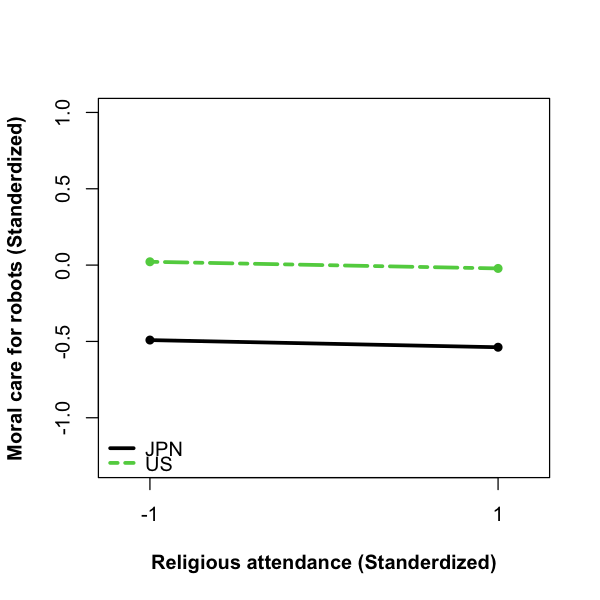
\includegraphics[width=8cm]{images/interaction_RA.png}}%
          \label{ra}
\subfloat[][宗教的信念と国籍の交互作用]{%
        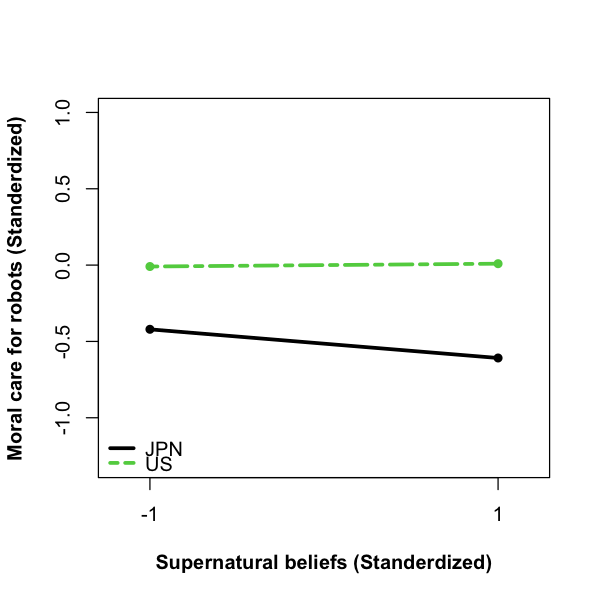
\includegraphics[width=8cm]{images/interaction_SBS.png}}%
          \label{sbs}
           \caption{交互作用の図示 (単純傾斜分析) }
           \label{fig:shayko}
       
\end{figure}


以上のことは、国籍との交互作用を考慮したことによって、当てはまり、予測力がともに向上したことを意味する。
モデルの係数を比較するとmodel 1aで存在した宗教的信念の主効果は、交互作用を考慮した場合は現れなかった。
以上より、仮説H2は支持された。ただし、残差の差、AICの差ともに小さく、交互作用の係数も大きくない ($|\beta| \sim .10$) ことから、弱い支持であるといえる。



\subsection{仮説H3、4:宗教がロボットに対する道徳に与える影響の構造}
仮説H3、H4を検証するために、multi-group SEMによるパスモデルへの当てはめを行った。仮説を表現したモデルは図\ref{hypot}に示している。具体的には、以下の4つの予測を検証した。
\begin{description}
\item{H3} 日本では、宗教性がアニミズムに正、人間中心主義に負の影響を持つ。逆にアメリカでは、宗教性が人間中心主義に正、アニミズムに負の影響を持つ。
\begin{description}
\item{i) } 宗教性は、日本ではアニミズムに正、アメリカではアニミズムに負のパス
\item{ii)} 宗教性は、日本では人間中心主義に負、アメリカでは人間中心主義に正のパス
\end{description}


\item{H4} どちらの国でも、ロボットに対する道徳的配慮に対して、アニミズムが正の、人間中心主義が負の影響を持つ。
\begin{description}
\item{iii)} 両方の国でアニミズムからロボットに対する道徳的配慮に正のパス
\item{iv)} 両方の国で人間中心主義からロボットに対する道徳的配慮に負のパス
\end{description}
\end{description}


係数の評価を行う前に、multi-group SEMによる当てはめに際して、両国のパス係数間に差異を仮定するかどうかを選択した。その方法は、両国でパス係数および回帰における切片が完全に異なるとしたモデル (model 2a) 、パス係数のみが異なるとしたモデル (model 2b) 、パス係数も切片も等しいとしたモデル (model 2c) を尤度の差の$\chi ^2$検定によって比較した。その結果、model 1aが最も良いモデルであると判断された (model 2a v. model 2b: $\Delta \chi ^2 = 406.2, \Delta df = 62, p < .0001$; model 2b v. model 2c: $\Delta \chi ^2 = 3177.5, \Delta df = 64, p < .001$) 。そのため、以下の評価はmodel 2aの結果をもとに行う。


仮説モデルに対して、許容できる当てはまりが得られた ( $\Delta \chi ^2(2510) = 8584.5, p = .000$, CFI = 0.96, RMSEA = 0.036 (95\%CI [0.035, 0.037]), GFI = 0.99, AGFI = 0.97;図\ref{fig:SEM}) 。




\begin{figure}[H]
  \centering
\subfloat[][仮説モデルへの当てはめ]{%
        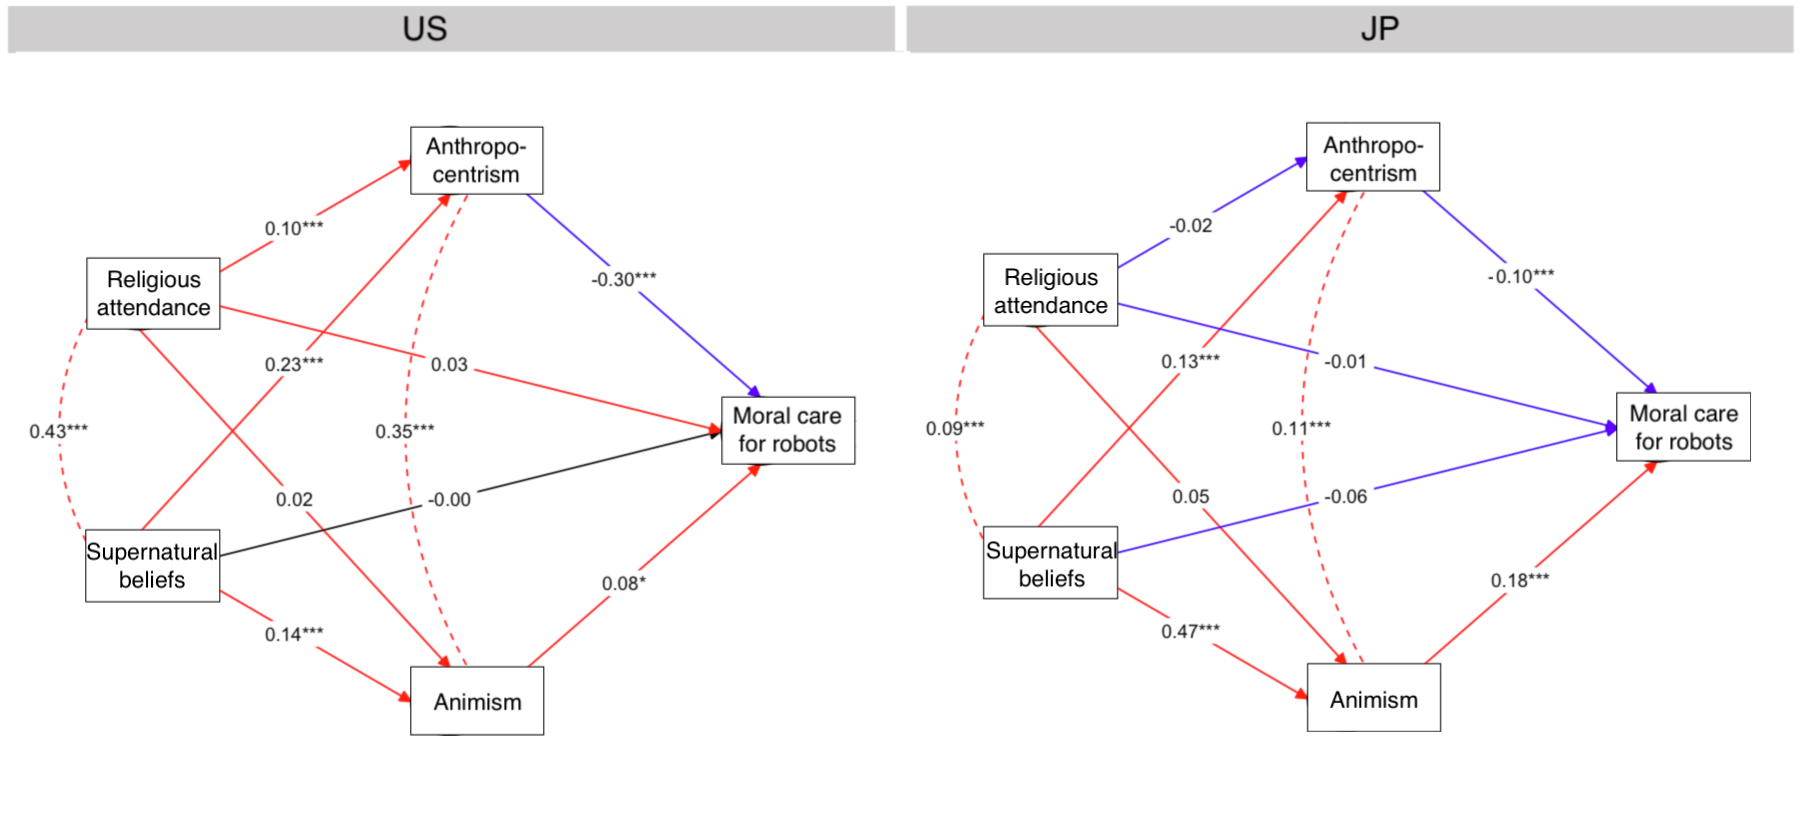
\includegraphics[width=16cm]{images/semImage.png}}%
          \label{subfig:sem}
\subfloat[][有意なパスのみを抽出した図]{%
        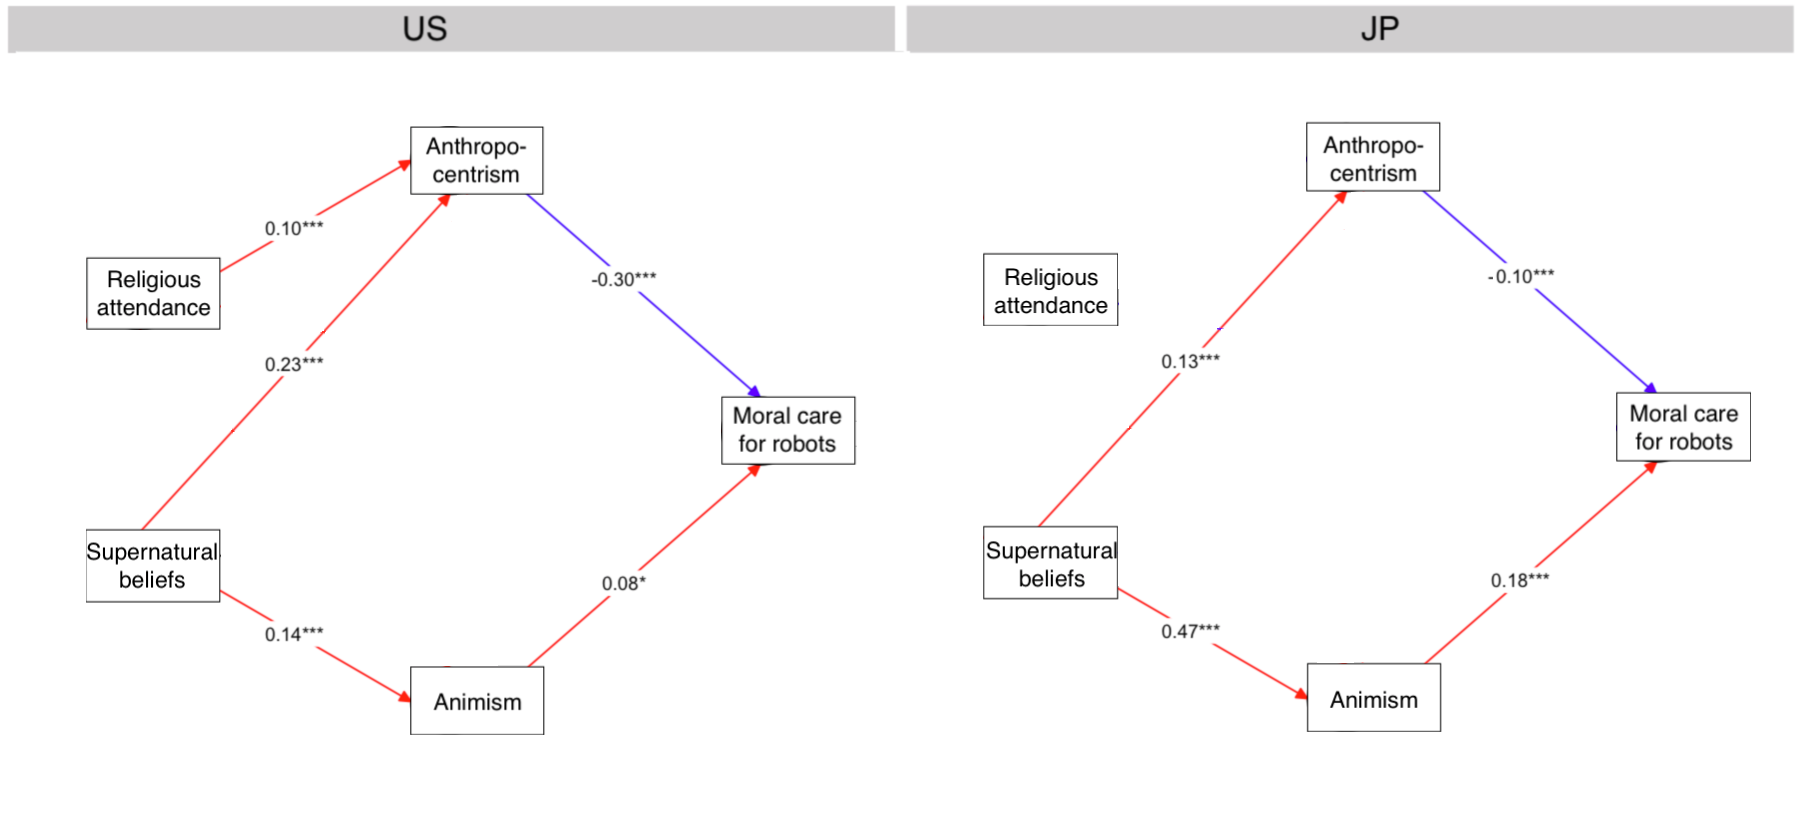
\includegraphics[width=16cm]{images/semImage_reduced.png}}%
          \label{subfig:red}
  \caption[multi-group SEMによる当てはめの図示]{multi-group SEMによる当てはめの図示。簡便のため、仮説に関係のない変数は図示していない。赤色のパスが正の、青色のパスが負の係数を表す。点線は残差の相関すなわち仮説モデルでは表現されていない変数間の関係を表す。測定変数、潜在変数、統制変数の間に相関を認めることで、仮説に関連する変数間の関係を抽出した。}
  \label{fig:SEM}
\end{figure}











%

\begin{table}[H]
{\scriptsize
  \begin{threeparttable}
\caption{multi-group SEMのパス係数}
\label{tab:Table_SEMp}
\begin{tabular}{@{}lllllll@{}}
\toprule
                                    &  & \multicolumn{2}{l}{US}        &  & \multicolumn{2}{l}{Japan}     \\ \cmidrule(lr){3-4} \cmidrule(l){6-7} 
                                    &  & β      & 95\%CI               &  & β      & 95\%CI               \\ \midrule
\textbf{回帰}                          &  &                               &                      &  &                               &                      \\
宗教への参加                &  &                               &                      &  &                               &                      \\
~~教育歴                       &  & ~0.54***                     & {[}~0.45, ~0.63{]} &  & ~0.17***                     & {[}~0.08, ~0.26{]} \\
~~ジェンダー                          &  & -0.23***                      & {[}-0.32, -0.14{]}   &  & -0.04                         & {[}-0.13, ~0.05{]}  \\
宗教的信念                &  &                               &                      &  &                               &                      \\
~~視点取得              &  & ~0.32***                     & {[}~0.26, ~0.37{]} &  & ~0.33***                     & {[}~0.28, ~0.39{]} \\
人間中心主義                    &  &                               &                      &  &                               &                      \\
~~宗教への参加            &  & ~0.10***                     & {[}~0.05, ~0.15{]} &  & -0.02                         & {[}-0.06, ~0.03{]}  \\
~~宗教的信念            &  & ~0.23***                     & {[}~0.18, ~0.29{]} &  & ~0.13***                     & {[}~0.08, ~0.17{]} \\
~~ジェンダー                          &  & -0.31***                      & {[}-0.39, -0.22{]}   &  & ~0.01                        & {[}-0.08, ~0.09{]}  \\
~~教育歴                       &  & ~0.15***                     & {[}~0.06, ~0.24{]} &  & -0.10*  & {[}-0.18, -0.01{]}   \\
アニミズム                             &  &                               &                      &  &                               &                      \\
~~宗教への参加            &  & ~0.14***                     & {[}~0.08, ~0.20{]} &  & ~0.47***                     & {[}~0.40, ~0.55{]} \\
~~宗教的信念            &  & ~0.02                        & {[}-0.03, ~0.07{]}  &  & ~0.05                        & {[}-0.00, ~0.10{]}  \\
ロボットに対する道徳的配慮               &  &                               &                      &  &                               &                      \\
~~宗教への参加            &  & ~0.03                        & {[}-0.02, ~0.09{]}  &  & -0.01                         & {[}-0.06, ~0.04{]}  \\
~~宗教的信念            &  & ~0.00                             & {[}-0.07, ~0.06{]}  &  & -0.06                         & {[}-0.13, ~0.00{]}  \\
~~アニミズム                         &  & ~0.08* & {[}~0.00, ~0.16{]} &  & ~0.18***                     & {[}~0.11, ~0.26{]} \\
~~人間中心主義           &  & -0.30***                      & {[}-0.36, -0.24{]}   &  & -0.09***                      & {[}-0.14, -0.04{]}   \\
~~擬人化傾向              &  & -0.16***                      & {[}-0.24, -0.08{]}   &  & ~0.14***                     & {[}~0.08, ~0.19{]} \\
~~共感的関心                &  & ~0.06                        & {[}-0.07, ~0.19{]}  &  & ~0.22* & {[}~0.08, ~0.36{]} \\
~~視点取得              &  & ~0.06                        & {[}-0.07, ~0.18{]}  &  & -0.08                         & {[}-0.22, ~0.05{]}  \\
~~ロボット関連メディア接触 &  & -0.25***                      & {[}-0.33, -0.18{]}   &  & -0.18***                      & {[}-0.25, -0.11{]}   \\
~~ジェンダー                          &  & ~0.35***                     & {[}~0.25, ~0.46{]} &  & ~0.41***                     & {[}~0.31, ~0.50{]} \\
~~教育歴                       &  & ~0.00                            & {[}-0.11, ~0.11{]}  &  & -0.20***                      & {[}-0.30, -0.10{]}   \\
ロボット関連メディア接触     &  &                               &                      &  &                               &                      \\
~~ジェンダー                          &  & -0.37***                      & {[}-0.47, -0.27{]}   &  & -0.04                         & {[}-0.15, ~0.07{]}  \\
~~教育歴                       &  & ~0.48***                     & {[}~0.35, ~0.60{]} &  & ~0.25***                     & {[}~0.11, ~0.39{]} \\
教育歴                           &  &                               &                      &  &                               &                      \\
~~ジェンダー                          &  & -0.23***                      & {[}-0.27, -0.18{]}   &  & -0.14***                      & {[}-0.18, -0.09{]}   \\
                                    &  &                               &                      &  &                               &                      \\
\textbf{残差の相関}                &  &                               &                      &  &                               &                      \\
SBS$\sim$$\sim$RA                   &  & ~0.43***                     & {[}~0.39, ~0.47{]} &  & ~0.09***                     & {[}~0.04, ~0.13{]} \\
RA$\sim$$\sim$AMO                   &  & ~0.07* & {[}~0.02, ~0.11{]} &  & ~0.04* & {[}~0.00, ~0.09{]} \\
RA$\sim$$\sim$EXP                   &  & ~0.18***                     & {[}~0.13, ~0.22{]} &  & ~0.25***                     & {[}~0.19, ~0.30{]} \\
SBS$\sim$$\sim$AMO                  &  & ~0.08***                     & {[}~0.04, ~0.13{]} &  & ~0.41***                     & {[}~0.37, ~0.45{]} \\
SBS$\sim$$\sim$EC                   &  & ~0.11***                     & {[}~0.06, ~0.15{]} &  & ~0.17***                     & {[}~0.12, ~0.22{]} \\
ANI$\sim$$\sim$ACE                  &  & ~0.35***                     & {[}~0.30, ~0.41{]} &  & ~0.11***                     & {[}~0.04, ~0.17{]} \\
ACE$\sim$$\sim$AMO                  &  & ~0.45***                     & {[}~0.40, ~0.49{]} &  & ~0.06* & {[}~0.02, ~0.09{]} \\
ANI$\sim$$\sim$AMO                  &  & ~0.60***                     & {[}~0.56, ~0.65{]} &  & ~0.30***                     & {[}~0.25, ~0.35{]} \\
ANI$\sim$$\sim$PT                   &  & ~0.20***                     & {[}~0.15, ~0.25{]} &  & ~0.38***                     & {[}~0.31, ~0.45{]} \\
ANI$\sim$$\sim$EC                   &  & ~0.18***                     & {[}~0.13, ~0.23{]} &  & ~0.32***                     & {[}~0.25, ~0.39{]} \\
EC$\sim$$\sim$PT                    &  & ~0.82***                     & {[}~0.78, ~0.86{]} &  & ~0.81***                     & {[}~0.76, ~0.85{]} \\
AMO$\sim$$\sim$EC                   &  & ~0.04                        & {[}-0.01, ~0.09{]}  &  & ~0.22***                     & {[}~0.17, ~0.27{]} \\
AMO$\sim$$\sim$PT                   &  & ~0.09***                     & {[}~0.04, ~0.13{]} &  & ~0.24***                     & {[}~0.20, ~0.29{]} \\
ACE$\sim$$\sim$EXP                  &  & ~0.32***                     & {[}~0.27, ~0.36{]} &  & ~0.21***                     & {[}~0.16, ~0.26{]} \\
ANI$\sim$$\sim$EXP                  &  & ~0.41***                     & {[}~0.36, ~0.45{]} &  & ~0.20***                     & {[}~0.13, ~0.26{]} \\
PT$\sim$$\sim$EXP                   &  & ~0.08***                     & {[}~0.05, ~0.12{]} &  & ~0.11***                     & {[}~0.07, ~0.15{]} \\
AMO$\sim$$\sim$EXP                  &  & ~0.53***                     & {[}~0.49, ~0.58{]} &  & ~0.16***                     & {[}~0.11, ~0.21{]}
\\ \bottomrule
\end{tabular}
    \begin{tablenotes}
      \small
      \item $^{*}$ ジェンダーおよび教育歴は2値変数として扱った。具体的にはジェンダー (0:男性、1:女性) 、教育歴 (1:大卒より長い教育歴、0:それ以外) 。MR:ロボットに対する道徳的配慮、RA:宗教への参加、SBS:宗教的信念、ACE:人間中心主義、ANI:アニミズム、AM:擬人化傾向、PT:視点取得、EC:共感的関心、EXP:ロボット関連メディア接触
      \item *$p < .05$. ***$p < .001$.
    \end{tablenotes}
  \end{threeparttable}
  }
\end{table}

\clearpage
%\thispagestyle{empty}


仮説モデルのパス係数と95\%信頼区間を表\ref{tab:Table_SEMp}に示した。
宗教的信念から人間中心主義、アニミズムへの効果を表したパスは、両国において正であった。
また、宗教への参加はアメリカで人間中心主義に正の効果を持っていたが、それ以外の効果は有意ではなかった。これらは予測 i) 、 ii) と合致しない。よって、仮説H3は支持されなかった。







パス係数の大きさを評価すると、日本においては宗教的信念からアニミズムのパス ($\beta=.47$) が人間中心主義へのパス ($\beta=.13$) よりも大きい。また、アメリカにおいては宗教的信念から人間中心主義のパス ($\beta=.23$) がアニミズムへのパス ($\beta=.14$) よりも大きい。よって、人間中心主義、アニミズムの相対的重要性では、仮説H3と同じ向きであった。



両国において、アニミズムからロボットに対する道徳的配慮のパスは正の係数、人間中心主義からロボットに対する道徳的配慮のパスは負の係数であった。これらはともに予測 iii) 、 iv) と合致する。よって、仮説H4は支持された。



二国間でのパス係数の比較を行ったところ、宗教的信念からアニミズムへのパスは日本 ($\beta=.47$) のほうがアメリカ ($\beta=.14$) より大きく、宗教的信念から人間中心主義へのパスはアメリカ ($\beta=.23$) のほうが日本 ($\beta=.13$) より大きかった。
また、アニミズムからロボットに対する道徳的配慮の正のパスは日本 ($\beta=.18$) のほうがアメリカ ($\beta=.08$) より大きかった。
尤度の差の検定の結果は表\ref{tab:SEMPathComp}に示した。
以上のことから、仮説モデルにおいて、日本ではアニミズムの影響が強く、アメリカでは人間中心主義の影響が強いことが示された。


\begin{table}[H]
\centering
\caption[パス係数の日米比較]{尤度の差の検定によるパス係数の日米比較}
\label{tab:SEMPathComp}
\begin{tabular}{@{}lllrl@{}}
\toprule
    固定したパス          & AIC       & $\chi^2$ & $\Delta \chi^2$ & p.value \\ \midrule
すべてのパスの違いを許容 & 949772.00 & 8584.46 & NA          & NA      \\
宗教への参加→人間中心主義   & 949780.10 & 8594.55 & 10.01  & 0.00    \\
宗教への参加→アニミズム & 949770.47 & 8584.92 & ~0.47  & 0.49    \\
宗教への参加→ロボットに対する道徳的配慮 & 949770.92 & 8585.37 & ~0.92  & 0.34    \\
宗教的信念→人間中心主義 & 949777.42 & 8591.87 & ~7.41  & 0.01    \\
宗教的信念→アニミズム & 949814.38 & 8628.83 & 44.37       & 0.00    \\
宗教的信念→ロボットに対する道徳的配慮 & 949771.85 & 8586.30 & ~1.85  & 0.17    \\
人間中心主義→ロボットに対する道徳的配慮 & 949793.50 & 8607.96 & 23.5       & 0.00    \\
アニミズム→ロボットに対する道徳的配慮 & 949773.16 & 8587.62 & ~3.16  & 0.08    \\ \bottomrule
\end{tabular}
\end{table}




\section{考察}
宗教および宗教に由来する価値観がロボットに対する道徳的配慮にどのように影響しているのかを明らかにするため、日本とアメリカの大規模サンプルを用いた文化比較調査を行った。


調査結果を以下にまとめる。まず、ロボットに対する道徳的配慮を比較したところ、日本のほうがアメリカよりもロボットに対する道徳的配慮が高いことが明らかになった (仮説H1支持) 。次に、宗教性がロボットに対する道徳的配慮に与える影響を検討した所、アメリカでのみ宗教的信念がロボットに対する道徳的配慮に負の影響を持つことが明らかになった (仮説H2部分的支持) 。


さらに、パスモデルによる分析の結果、日本とアメリカで共通する構造が明らかになった。
すなわち、人間中心主義とアニミズムは宗教的信念からともに正の影響を受けていた (H3不支持) 。そして、ロボットに対する道徳的配慮に対して、アニミズムは正の、人間中心主義は負の影響を与えていた (仮説H4支持) 。すなわち、ロボットに対する道徳的配慮に相反する影響を与える2つの価値観に対して、宗教が正の影響を与えるという構造が両国で見いだされた。


以下では、それぞれの発見を先行研究の報告に即して考察する。

\subsection{ロボットに対する道徳的態度に現れた文化差}
これまでにも、日本とアメリカを比較した研究\cite{mania}において、日本ではアメリカよりも、ロボットに対して暖かい印象が持たれ、好まれやすいという結果が報告されている。また、日本ではイギリスに比べてロボットに対する否定的態度が弱いという結果も報告されている\cite{humuk} 。ロボットに対する道徳的配慮が日本でアメリカより高いという本研究の結果は、西洋より日本のほうがロボットに対して親和的であるというこれらの報告と符合する。それに加え本研究では、アメリカでのみ宗教的信念がロボットに対する道徳的配慮に負の影響を与えることが明らかになった。


これに加え、本研究では人間中心主義とアニミズムという宗教に由来する価値観の影響を考慮した解析を行った。これらは理論的\cite{mania, gygi}、あるいは実証的\cite{okanda}な先行研究においてロボットに対する態度を左右する可能性が指摘されていた価値観である。本研究はこれらの価値観がロボットに対する態度に与える影響を、国際比較調査において初めて検証した。
このような理論に基づく文化比較研究はロボットに対する態度の研究において重要性が指摘されている\cite{review} 。人間中心主義、アニミズムとロボットに対する道徳的配慮に理論的予測に合致する関係が見られたことから、宗教に由来する価値観はロボットに対する態度を左右する要因になりえることが示された。
さらに、2つの価値観が与える影響の正負が日本とアメリカで共通していたことから、これら2つの価値観の組み合わせによって、より広い文化圏に対して当てはまる理論が構築できる可能性がある。


本研究の発見は、理論的貢献のみならず、工学的な分野でのインタラクションデザインに対する示唆も与えると考えられる。
例えば、ソーシャルロボットに対する攻撃 (いわゆるロボットいじめ\cite{ijime}) をやめさせる戦略を考える際、アニミズム傾向が高い国では、ロボットが同情心を喚起するような発話を行うことで、通りすがりの人にいじめを止めさせるアプローチが有効だと考えられる。逆に、人間中心主義傾向が高い国では、ロボットがいかに高価であるか、破壊された場合の賠償がいくらであるかといった人間社会での尺度をベースにした発話のほうがいじめをやめさせるのに有効であるかもしれない。

さらに、人間中心主義とアニミズムを目的変数として、特定のインタラクションデザインに対する選好を調べるアプローチも有効であるかもしれない。人間中心主義傾向の高い人に対してはロボットは擬人的に振る舞うのではなくより機械らしく振る舞うほうが好まれると行った結果が得られる可能性がある。このような、文化的背景を考慮した ``culture aware''\cite{cultu} なインタラクションデザインの重要性が近年指摘されている。


\subsection{宗教心の測定方法による影響}
本研究では、宗教への参加と宗教的信念という2つの観点から宗教性を測定していた。このうち、 (直接or宗教に由来する価値観を媒介して) ロボットに対する道徳的配慮に影響を与えていたのは、宗教的信念のみであった。
日本の宗教においては信念よりも参加が顕著であるため\cite{kava}、宗教への参加が影響力を持つ可能性が考えられたが、この可能性は支持されなかった。


宗教への参加が影響力を持たなかった理由として、宗教への参加が個人の価値観とは別の要素で促進される場合があることが考えられる。日本の宗教的慣習を調査した研究\cite{kava}では、葬儀などの特別な用事がある場合のみ宗教施設を訪れると回答した割合が26\%であり、年に1度しか訪れない人も19\%存在した。さらに、多くの場合宗教施設を訪れる理由は特定の教義の信仰ではなく、観光目的や家族・友人のために祈る目的であった。このように日本では、宗教施設に行くこと (今回測定した宗教への参加) は、特定の信念や価値観 (たとえばアニミズムや人間中心主義) と結びつくものではない可能性がある。同様に、アメリカにおいても教会への出席は社会的規範によって促進されることが報告されている\cite{church} 。

\subsection{宗教に動機づけられた価値観とロボットに対する道徳的態度の関係}
宗教的信念は、両国において人間中心主義、アニミズムの両方に対して正の影響を持っていた。日本において宗教的信念が人間中心主義に正の影響を持っていたことと、アメリカにおいてアニミズムに正の影響を持っていたことは、これまでなされてきた理論的主張\cite{hosaka}と合致しない。
宗教の認知科学\cite{csr}の分野では、特定の心理的態度や行動が複数の宗教で現れることが指摘されている\cite{jong} 。このことを踏まえると、宗教的信念が人間中心主義、アニミズムの両方に対して正の影響を持つという結果は、今回対象とした2つの宗教においてこれら2つの価値観は共有されていたものである可能性がある。宗教が人間中心主義とは相反すると予測されていた日本でも実際には正の関係が見られたことは、教えの内容は違えど宗教自体は人間が生み出したものであるという事実を反映しているのかもしれない。しかし、これらの結果の背後にあるメカニズムは未知であるため、宗教と宗教に由来する価値観が複数の文化圏でどのように結びついているのかをより詳しく理解するためにはさらなる研究が必要である。


一方で、アニミズムおよび人間中心主義とロボットに対する道徳的配慮の関係は、既存の議論と一貫する結果であった。
日本の成人を対象とした研究で、ロボットに対する共感が、アニミズムと正の関係を持つことが報告されている\cite{okanda} 。本研究で見いだされたアニミズムとロボットに対する道徳的配慮の正の関係は、この報告と合致する。同様に、キリスト教圏 (イタリア) の調査で、人間中心主義がロボットに対する否定的態度と正の相関を持つという結果も報告されている\cite{fortu}が、本研究で見いだされた人間中心主義とロボットに対する道徳的配慮の負の関係もこれと合致する。
本研究は、これらの先行研究に基づき国際比較調査を行うことで、ロボットに対する態度と宗教的伝統の関係をより深く明らかにした。具体的には、人間中心主義とアニミズムという宗教に由来する価値観が、異なる宗教的伝統の影響下でも同じようにロボットに対する態度に影響することが明らかになった。一方で、影響力の大きさには二国間での違いも見いだされた。


\subsection{文化差の構造}
ロボットに対する道徳的配慮の強さは、日本のほうがアメリカよりも強く、アメリカでは宗教的信念と負の関係を持っていた。人間中心主義、アニミズムを考慮した解析によって、この文化差がどのように生じているのかを詳細に検討した。その結果、日本とアメリカで共通する構造が発見された。具体的には、宗教的信念が人間中心主義とアニミズムに正に影響し、ロボットに対する道徳的配慮に対してアニミズムは正の、人間中心主義は負の影響するという構造である。すなわち、ロボットに対する道徳的配慮における文化差は、宗教や宗教に由来する価値観の間に異なる構造があることから生じているのではなかった。むしろ、それぞれの間の影響力の相対的な大きさの違いが文化差を生じさせていた。


人間中心主義とアニミズムは、どちらも宗教的信念から正の影響を受けつつも、ロボットに対する道徳的配慮に相反する影響を与えていた。すなわち、2つの逆向きの媒介効果が打ち消し合っていたと考えることができる。日本においては、アニミズムによる正の影響のほうが顕著であり、アメリカでは人間中心主義による負の影響のほうが顕著であった。アメリカでのみ宗教的信念がロボットに対する道徳的配慮に負の影響を持っていたことは、アメリカでのみ、2つの媒介効果のうち人間中心主義の影響が卓越していたことを示唆する。


態度や信念に現れる文化差の背景に、このような相反する要素の相対的重要性の違いが存在するという可能性は、見知らぬ他者を信頼する傾向に現れる文化差を説明する理論\cite{yamagishi}でも指摘されている。この理論では、集団内の相互監視システムを参照して他者を信頼するかを判断する戦略と、集団に依存せず信頼に足る相手かどうかを判断する戦略が対置される。実証研究においても、日本では前者、アメリカでは後者が卓越することが示されている。

\subsection{補助的考察}
本小節では、今回検討した仮説とは直接関連しない結果について議論する。
測定した変数の記述統計量およびそれらの相関行列は表\ref{tab:Table_Desc}と表\ref{tab:Table_Cor_JP}、表\ref{tab:Table_Cor_US}に示した。



宗教への参加に関しては、アメリカのほうが頻度が高いという結果が得られた ($t(3154.5) = -22.9, p = .000$) 。宗教的信念についても同様に、アメリカのほうが高かった ($t(3770.5) = -32.8, p = .000$) 。
これらは、日米の宗教態度の比較を行った先行研究と合致する結果である\cite{kava} 。



アニミズム傾向に関して、文化の影響は見られなかった ($t(3519) = -0.52, p = .600$) 。人間中心主義では、アメリカのほうが高いという文化差が見られた ($t(3436.4) = -10.4, p = .000$) 。
これまでの社会学での議論では、日本は西洋に比べアニミズム傾向が高いという主張がなされてきた\cite{hosaka}が、この結果はそれとは合致しない。このことが原因となって、仮説H3が支持されなかった可能性がある。一方で、人間中心主義がアメリカのほう高いという結果は、既存の議論\cite{abe}と合致する結果である。


他者の視点取得、共感的関心においては、どちらもアメリカのほうが日本より高いという結果になった (それぞれ$t(3577.6) = -20.3, p = .000$;$t(3514.7) = -28.4, p = .000$) 。よって、日本のほうがロボットに対する道徳的配慮が高いという結果は、日本のほうが「他人のネガティブな経験に対していつも生じる感情的反応」が強いことによってもたらされたものではないと結論できる。


回帰分析、パス解析において、男性以外のジェンダーを回答した実験参加者のほうが、ロボットに対する道徳的配慮が高いという結果が現れていた (回帰分析で$\beta=0.28$) 。このことは女性がよりロボットに対して親和的であるという既存の知見\cite{gend, gend2}と一致する結果となった。また、回帰分析において擬人化傾向と国籍の交互作用が有意であった ($\beta=-.27$;主効果は$\beta=.15$) 。この結果は、日本では擬人化傾向はロボットに対する道徳的配慮に正の影響を持つのに対して、アメリカでは負の影響を持つことを意味する。すなわち、日本とアメリカでは、擬人化傾向がロボットに対する道徳に与える影響が異なる可能性を示唆する。日米で「擬人化されたエージェント」の捉え方が異なることを示しているのかもしれない。この点については本研究から結論を出すことはできないため、今後の研究が必要である。

\subsection{留意事項}
今回行った分析では、ロボットに対する道徳的配慮と人間に対する道徳的配慮の関係は検討しなかった。そのため、ロボットに対してのみ向けられる道徳的配慮が人間に対する道徳的配慮から分離できていなかった可能性がある。ただし、本研究では他者の痛みを感じる能力 (Empathic concern) を統制している。また、本研究の関心は、ロボットと人間に対する道徳的配慮の差ではなく、ロボットに対する道徳的配慮そのものであることから、今回の実験デザインは妥当であったと考えている。一方で、ロボットと人間に対する道徳的配慮の差を検討することも興味深いテーマであるため、今後このような方向性に研究を発展させることも意義があると考えられる。例えば、ロボットに対するいじめを見た場合に、人に対するいじめを見たときと類似した神経活動が見られるという知見\cite{fmri}が報告されているが、このような反応の個人差にアニミズムや人間中心主義は影響しているのだろうか、といった問いを立てて研究することが可能である。



また、「ロボット」という対象一般に対する道徳的配慮に関心を持っていたことから、本研究では提示する刺激に特定のロボットが害を与えられる映像を用いず、「ロボット」という言葉を含む文章を提示し、その\kenten[s]{受け入れられなさ}を測定した。そのため、実験参加者が「ロボット」としてどのような対象を想定したかによって結果が影響された可能性がある。ただし、その影響を抑えるために、実験参加者が質問紙に回答する際に、3体のロボット (Armar、HRP-2、Nao;図\ref{fig:Robots}(a)) が示された画像を提示し、それらを「ロボット」として思い浮かべるよう教示した。これらの提示したロボットは、予備実験において日本と西洋 (アメリカ、イギリス、カナダ) の評定者に「人間らしさ」が同程度であり、感情的印象\footnote{ロボットの見た目によってどれだけポジティブな感情が喚起されるかを、言語に依存しない感情測定指標であるSelf-Assessment Manikin (SAM \cite{sam}) によって評定させた。}が近いと判断されたロボットの画像\cite{ikari}を用いた。以上のことから、本研究の結果が、ロボットの画像が喚起した感情的印象の差異によって引き起こされたとは考えづらい。


本研究で扱った道徳はCare基盤のみであるため、Fairnessのような他の基盤に拡張して研究することで、ロボットに対する道徳的態度のさらなる包括的な理解が可能になると期待できる。インタラクションデザインの評価を目的として、ロボットと財を分配するという状況下での人の行動を計測する実験は行われている\cite{fairness} 。しかし、そのような状況下での判断に、人の宗教的バックグラウンドが及ぼす影響は評価されていない。
さらに、今回調査した国は日本とアメリカのみである。アメリカと同様にユダヤ・キリスト教圏であるヨーロッパの国々や、同じ啓示宗教ではあるがキリスト教とは異なった歴史を持つイスラム圏などを対象とした研究が考えられる。同様に日本との共通点もあるが、儒教の影響の強い中国や韓国といった国を研究することも興味深い。このように複数の文化圏で同様の実験パラダイムによる追試を行うことで、「ロボットに対する道徳を促進するアニミズム」と「抑制する人間中心主義」という2つの価値観に着目したアプローチの妥当性が検証できる。



本研究は質問紙調査であるため、このことに起因する制限事項が存在する。まず、実際の状況において人が、質問紙に回答した内容と一貫した行動を取るのかは未知である。ロボットに対して攻撃をする人が許せないと感じたとしても、それを止めるような行動を取るかどうかは、ロボットに対する態度のみならず、その人の性格や社会的状況によっても影響されるはずである。この点を実験室実験によって検証することで、工学的により応用可能性が高い知見が得られると期待できる。



%% Chapter 4
\newpage
\chapter{人間以外の存在に対する道徳と宗教}
本研究で着目したロボットに対する道徳的配慮は、人間以外に対する道徳というテーマの一つであると考えることができる。本章では、本研究の結果を、人間以外に対する道徳を扱った先行研究と対応させて論じる。

\section{人間以外に対する道徳:Moral circle approachからの解釈}
人間以外に対する道徳を扱う際に用いられる概念の一つに、Moral circle \cite{singer}がある。Moral circleとは、人が道徳を適用する範囲のことである。人の歴史上、Moral circleの範囲は拡大していることが指摘されている\cite{lecky, singer} 。例えば、奴隷制が廃止されたことにより、それまで道徳の対象外 (すなわちMoral circleの外側の存在) であったとみなされていた人が道徳の対象となった。さらに近年では、動物が道徳の対象とみなされるケースも現れている。


Moral circleを扱う研究者たちは、道徳適用の範囲の広さがどのような要因によって規定されるのかを調査してきた。このアプローチでは、家族、友人、異国人、地球環境、動物、昆虫、植物といった対象に対して道徳心を覚えるかどうかを尋ね、どれだけの対象が含まれるかを定量化する。
このアプローチでは、道徳適用を行うかどうかを測定する際に、それを守るべきという責務を感じるかをという基準が頻繁に用いられる。例えば、``circle those that you feel morally obligated to show concern for'' (それらに対して気にかける道徳的責務を感じる対象を囲んでください;筆者訳) \cite{laham}といった質問項目が用いられている。この基準による道徳の測定は道徳基盤理論におけるCare基盤で示されている道徳と概念的に類似している。実際、Moral circleと道徳基盤の関係を調査した研究では、Care基盤とMoral circleの広がりが正に相関することが示されている\cite{crim} 。


以上のことから、本研究では「ロボットをMoral circleに含めるかを調査した」とみなすことも可能である (ただし、Moral circle approachをとる先行研究では、通常は道徳適用の対象か否かを2択で選択させるため、本研究の手法はどれだけロボットをMoral circleに含めるかの程度を測定したことに相当すると考えられる) 。このように考えると、本研究の結果は道徳適用の範囲の広がりに宗教や宗教に由来する価値観が影響する可能性を示すと解釈できる。これまでの研究では、イデオロギー\cite{ideo}や自分の道徳性に対する自信\cite{jishin}がMoral circleの広がりが影響することが報告されているが、宗教を扱ったものは筆者の知る限りでは存在しない。また、ロボットのような人工エージェントを対象にした研究もほとんど存在しない。ゆえに、本研究の結果はMoral circle研究に対しても示唆をもたらすと考えられる。
%Reed, A., & Aquino, K. F. (2003). Moral identity and the expanding circle of moral regard toward out-groups. Journal of Personality and Social Psychology, 84(6), 1270\UTF{2013}1286. doi:10.1037/0022-3514.84.6.1270\UTF{00A0}%

\section{宗教の影響}
宗教が非人間に対する道徳や倫理に影響を与える可能性は複数の研究者によって指摘されている\cite{ecocen, white_, jaga, ser} 。%(Jegatheesan, 2015). Serpell (2005) Washington et al. (2017) 
%White, L. (1967). The historical roots of our ecological crisis. Science, 155, 1203\UTF{2013}1207.
すなわち、動植物のような非人間が価値体系の中でどのように位置づけられるのか、またそれらに対してどのように接するべきかは、宗教的伝統によって規定されてきた\cite{jaga} 。それどころか、動植物のような自然を人の利益のために傷つけることは許されることなのかというジレンマが宗教的伝統の形成に影響を与えていることも指摘されている\cite{ser} 。さらには、西洋で行われてきた自然環境の搾取の背景には、人間を特別な存在であるとみなす宗教的伝統の影響があると論じる研究者もいる\cite{white_} 。



実証研究が行われた例としては、環境保護に関する調査が存在する (詳細にはレビュー\cite{proen}を参照) 。例えば、米国で行われた調査において、保守的なプロテスタントや聖書の信奉者は、そうでない人に比べて環境保護に対する意欲が低く、コストを払うことに対しても消極的であるという結果が報告されている\cite{ameri} 。同様に、複数の国を対象とした研究でも、聖書に対する信仰が強い人は環境に対する危惧が薄く、人間中心主義的な動機 (=環境が損なわれることによって人間に対する害が起きることを危惧する) によって環境問題に対する関心を持っていることが明らかになっている\cite{multi} 。
% https://onlinelibrary.wiley.com/doi/abs/10.1111/j.1468-5906.2007.00341.x
%レビュー:  https://onlinelibrary.wiley.com/doi/full/10.1002/ijop.12034
%(Schultz, Zelezny & Dalrymple, 2000)
% stewardshipを通じて正に影響するケースもある(神の恵みを正しく持続的につかわなければならない)
本研究の結果も、宗教が非人間に対する道徳を左右する可能性を示す一例と考えることができる。ロボットのような人工エージェントに対する道徳を扱った研究はほとんど存在しないことから、本研究の発見は他にも、様々な発展の可能性を持つと考えられる。





% 道徳は義務論的な概念
% どんなものに対して適用されるかというのも、じつは宗教の影響を受けている
% ロボットについてこのことを明示して扱った研究は少ない
% したがって、文化差を考慮してrobot rightsを扱おうという動きは、重要性の指摘はあるものの、影響力を持っていなかった
% 


\section{人工エージェントに対する道徳:本研究がもたらす示唆}
ロボットという人工エージェントを対象に、宗教が道徳に与える影響やその文化差を実証的に検証したことで、人工エージェントに対する道徳・倫理という現代の倫理学のトピックに対する示唆が得られた。
「人工エージェントに対する態度が道徳的に拘束されるべきか」という問いは、昨今の倫理学的議論で取り上げられている\cite{whitby} 。その理由の一つは、人工エージェントを道徳の対象ではない存在として扱う態度が、人間に対する権利の侵害へと繋がる可能性があるからである\cite{sex} 。このような倫理学的問題に対して、様々な形で理論的な解決が試みられている\cite{coeck, danaha} 。しかし、これまでに国際的な合意や、具体的なガイドラインのような成果は生まれていない。本研究のように文化の違いを考慮に入れた実証的研究を行うことで、様々な文化圏で、人工エージェントに対する道徳・倫理に関する理論的な提案が、人々が実際に感じる道徳心とどれだけ合致するかを検証することが可能になる。その結果、さまざまな文化圏に対して実効性がある実践的な枠組みを策定することに繋がると考えられる。本研究の結果からは、少なくとも人工エージェントに対する道徳・倫理を議論する上では、宗教的伝統といった文化の影響を無視することができないという示唆が得られた。実際、日本において外国人労働者よりもロボットがより優先的に道徳的な配慮の対象とされているという事例が報告されている\cite{immig} 。このように人工エージェントに関する道徳・倫理は、文化を考慮して取り組むべき問題であると考えられる。

% 1)robot rights, rights for agentsに新たな方向性
% 宗教による違いを前提にガイドラインを作る

% 2)人工エージェントに対する道徳がどうきまるのかをいろんな対象を使って深堀りできる


%% Chapter 5
\newpage
\chapter{結論}
宗教や宗教に由来する価値観がロボットに対する道徳的態度にどのような影響を与えるのかを日本とアメリカの大規模サンプルを用いて調査した。道徳性の中でも、ロボットが害を受けることをどれだけ許せないか (道徳的配慮) に着目し、宗教を動機とする価値観がロボットに対する道徳的配慮にどのような影響を与えるかに注目する新規なアプローチを行った。その結果、人間中心主義とアニミズムという2つの宗教的価値観が、ロボットに対する道徳的配慮に対して互いに逆の影響を及ぼすという、日米共通の構造が明らかになった。
研究の成果は、文化の違いを考慮したロボットのインタラクションデザインのみならず、人工エージェントに対する道徳・倫理に関する研究にも貢献すると考えられる。





\renewcommand{\bibname}{引用文献}
\addcontentsline{toc}{chapter}{引用文献}
\begin{thebibliography}{999}
\bibitem{spot} Parke, P. (2015, February 13) Is it cruel to kick a robot dog?. \textsl{CNN}. \url{https://edition.cnn.com/2015/02/13/tech/spot-robot-dog-google/index.html}
\bibitem{hitch} Fraser, K. C., Zeller, F., Smith, D. H., Mohammad, S., \& Rudzicz, F. (2019, June). How do we feel when a robot dies? Emotions expressed on Twitter before and after hitchBOT’s destruction. In \textsl{Proceedings of the Tenth Workshop on Computational Approaches to Subjectivity, Sentiment and Social Media Analysis.} 62-71. \url{http://dx.doi.org/10.18653/v1/W19-1308}
\bibitem{abuse} Bartneck, C., \& Keijsers, M. (2020). The morality of abusing a robot. \textsl{Journal of Behavioral Robotics, 11}(1), 271-283. \url{https://doi.org/10.1515/pjbr-2020-0017}
\bibitem{coeck} Coeckelbergh, M. (2018). Why care about robots? Empathy, moral standing, and the language of suffering. \textsl{Kairos. Journal of Philosophy \& Science, 20}(1), 141-158. \url{https://doi.org/10.2478/kjps-2018-0007}
\bibitem{phobia} Halpern, D., \& Katz, J. E. (2012). Unveiling robotophobia and cyber-dystopianism: The role of gender, technology and religion on attitudes towards robots. In \textsl{2012 7th ACM/IEEE International Conference on Human-Robot Interaction (HRI)} (pp. 139-140). IEEE. \url{https://doi.org/10.1145/2157689.2157724}
\bibitem{mania} MacDorman, K. F., Vasudevan, S. K., \& Ho, C. C. (2009). Does Japan really have robot mania? Comparing attitudes by implicit and explicit measures. \textsl{AI \& society, 23}(4), 485-510. \url{https://doi.org/10.1007/s00146-008-0181-2}
\bibitem{social} Shaw-Garlock, G. (2009). Looking forward to sociable robots. \textsl{International Journal of Social Robotics, 1}(3), 249-260. https://doi.org/10.1007/s12369-009-0021-7 
\bibitem{review} Papadopoulos, I., \& Koulouglioti, C. (2018). The influence of culture on attitudes towards humanoid and animal‐like robots: an integrative review. \textsl{Journal of Nursing Scholarship, 50}(6), 653-665. \url{https://doi.org/10.1111/jnu.12422}
\bibitem{roboeth} Sullins, J. P. (2011). Introduction: Open questions in roboethics.
\textsl{Philosophy \& Technology, 24}, 233-238. \url{http://dx.doi.org/10.1007/s13347-011-0043-6}
\bibitem{moralrobo} Malle, B. F. (2016). Integrating robot ethics and machine morality: the study and design of moral competence in robots. \textsl{Ethics and Information Technology, 18}(4), 243-256. \url{http://dx.doi.org/10.1007/s10676-015-9367-8}
\bibitem{sex} Danaher, J. (2017). Robotic rape and robotic child sexual abuse: should they be criminalised?. \textsl{Criminal law and philosophy, 11}(1), 71-95. \url{https://doi.org/10.1007/s11572-014-9362-x}
\bibitem{when}  Shevlin, H. (2021). How Could We Know When a Robot was a Moral Patient?. \textsl{Cambridge Quarterly of Healthcare Ethics, 30}(3), 459-471. \url{https://doi.org/10.1017/S0963180120001012}
\bibitem{Darling} Darling, K. (2016). Extending legal protection to social robots: The effects of anthropomorphism, empathy, and violent behavior towards robotic objects. In \textsl{Robot law}. Edward Elgar Publishing. \url{http://dx.doi.org/10.2139/ssrn.2044797}
\bibitem{Kant} Kant, I. (2001). \textsl{Lectures on ethics (Vol. 2)}. Cambridge University Press.
\bibitem{white} McKay, R., \& Whitehouse, H. (2015). Religion and morality. \textsl{Psychological Bulletin, 141}(2), 447-473. \url{http://dx.doi.org/10.1037/a0038455}
\bibitem{MFT} Graham, J., Haidt, J., Koleva, S., Motyl, M., Iyer, R., Wojcik, S., \& Ditto, P. (2013). Moral foundations theory: The pragmatic validity of moral pluralism. \textsl{Advances in Experimental Social Psychology, 47}, 55-130. \url{https://doi.org/10.1016/B978-0-12-407236-7.00002-4}
\bibitem{jpmft} Matsuo, A., Sasahara, K., Taguchi, Y., \& Karasawa, M. (2019). Development and validation of the Japanese moral foundations dictionary. \textsl{PloS one, 14}(3), e0213343. \url{https://doi.org/10.1371/journal.pone.0213343}
\bibitem{frmft} M\`{e}tayer, S., \& Pahlavan, F. (2014). Validation de l’adaptation Fran\c{c}aise du Questionnaire des principes Moraux Fondateurs [Validation of the Moral Foundations Questionnaire in French]. \textsl{Revue Internationale de Psychologie Sociale, 27}(2), 79-107.
\bibitem{mfcr} Graham, J., Nosek, B. A., Haidt, J., Iyer, R., Koleva, S., \& Ditto, P. H. (2011). Mapping the moral domain. \textsl{Journal of Personality and Social Psychology, 101}(2), 366-385. \url{https://doi.org/10.1037/a0021847}
\bibitem{ideo_} Graham, J., Haidt, J., \& Nosek, B. A. (2009). Liberals and conservatives rely on different sets of moral foundations. \textsl{Journal of personality and social psychology, 96}(5), 1029-1046. \url{https://doi.org/10.1037/a0015141}
\bibitem{tro} Malle, B. F., Scheutz, M., Forlizzi, J., \& Voiklis, J. (2016, March). Which robot am I thinking about? The impact of action and appearance on people's evaluations of a moral robot. In \textsl{2016 11th ACM/IEEE International Conference on Human-Robot Interaction (HRI) (pp. 125-132).} IEEE. \url{https://doi.org/10.1109/HRI.2016.7451743}
\bibitem{appe} Nijssen, S. R., M\"{u}ller, B. C., Baaren, R. B. V., \& Paulus, M. (2019). Saving the robot or the human? Robots who feel deserve moral care. \textsl{Social Cognition, 37}(1), 41-56. \url{https://doi.org/10.1521/soco.2019.37.1.41}
\bibitem{paro} Shibata, T., Wada, K., \& Tanie, K. (2004, April). Tabulation and analysis of questionnaire results of subjective evaluation of seal robot in Japan, UK, Sweden and Italy. In \textsl{IEEE International Conference on Robotics and Automation, 2004. Proceedings. ICRA'04. 2004} (Vol. 2, pp. 1387-1392). IEEE. \url{https://doi.org/10.1109/ROBOT.2004.1308018}
\bibitem{humuk} Nomura, T., Syrdal, D. S. \& Dautenhahn, K. (2015). Differences on social acceptance of humanoid robots between Japan and the UK. In \textsl{Proceedings of the 4th International Symposium on New Frontiers in Human Robot Interaction} (pp. 115-120). Bath, UK: AISB.
\bibitem{argen} Joosse, M. P., Poppe, R. W., Lohse, M., \& Evers, V. (2014, August). Cultural differences in how an engagement-seeking robot should approach a group of people. In \textsl{Proceedings of the 5th ACM international conference on Collaboration across boundaries: culture, distance \& technology} (pp. 121-130). \url{https://doi.org/10.1145/2631488.2631499}
\bibitem{german} Li, D., Rau, P. L. P., \& Li, Y. (2010). A cross-cultural study: Effect of robot appearance and task. \textsl{International Journal of Social Robotics, 2}(2), 175-186. \url{https://doi.org/10.1007/s12369-010-0056-9}
\bibitem{aibo} Bartneck, C., Suzuki, T., Kanda, T., \& Nomura, T. (2007). The influence of people’s culture and prior experiences with Aibo on their attitude towards robots. \textsl{Ai \& Society, 21}(1-2), 217-230. \url{http://dx.doi.org/10.1007/s00146-006-0052-7}
\bibitem{bunseki} Ji, L.-J., Peng, K., \& Nisbett, R. E. (2000). Culture, control, and perception of relationships in the environment. \textsl{Journal of Personality and Social Psychology, 78}(5), 943-955. \url{https://doi.org/10.1037//0022-3514.78.5.943}
\bibitem{four} Mazlish B (1993) \textsl{The fourth discontinuity: the co-evolution of humans and machines.} Yale University Press, New Haven.
\bibitem{gygi} Gygi, F. R. (2018). Robot companions: The animation of technology and the technology of animation in Japan. In Astor-Aguilera, M., \& Harvey, G. (Eds.), \textsl{Rethinking Relations and Animism} (1st ed., pp. 94-111). Routledge. \url{https://doi.org/10.4324/9780203709887}
\bibitem{eye} Reinhardt, M. (1972). Anthropocentrism. In Eysenck, H.J., Arnold, W., \& Meili, R. (Eds.) \textsl{Encyclopedia of psychology} (\textsl{Vol. 1}, p. 62). Herder KG, West Germany.
\bibitem{chand} Chandler, E. W. (1981). Anthropocentrism: Construct validity and measurement \textsl{[Doctoral dissertation, Louisiana State University and Agricultural \& Mechanical College]}.
\bibitem{kozoku} Vakoch, D. A., \& Lee, Y. S. (2000). Reactions to receipt of a message from extraterrestrial intelligence: A cross-cultural empirical study. \textsl{Acta Astronautica, 46}(10-12), 737-744. \url{http://dx.doi.org/10.1016/S0094-5765(00)00041-2}
\bibitem{fortu} Fortuna, P., Wr\'{o}blewski, Z., \& Gorbaniuk, O. (2021). The structure and correlates of anthropocentrism as a psychological construct. \textsl{Current Psychology: A Journal for Diverse Perspectives on Diverse Psychological Issues.} Advance online publication. \url{https://doi.org/10.1007/s12144-021-01835-z}
\bibitem{hisimage} Melchert, C. (2011). God Created Adam in His Image. \textsl{Journal of Qur'anic Studies, 13}(1), 113-124. \url{https://doi.org/10.3366/jqs.2011.0009}
\bibitem{abe} Abe, M. (1997). Shinto and Buddhism: The two major religions of Japan. In Steven, H. (Ed.), \textsl{Zen and comparative studies} (pp. 221-231). Palgrave Macmillan. \url{https://doi.org/10.1057/9780230375994_16}
\bibitem{james} James, S. P. (2004). \textsl{Zen Buddhism and environmental ethics (1st ed.)}. Routledge.
\bibitem{rots} Rots, A. P. (2017). Public shrine forests? Shinto, immanence, and discursive secularization. \textsl{Japan Review, 30}, 179-205.
\bibitem{catho} Oliveira, A. J. de. (2020). Technology use in the conservative family context. \textsl{RTIC - Revista De Tecnologias, Informa\c{c}\~{a}o E Comunica\c{c}\~{a}o, 1}(1), 49-59. Obtido de. \url{https://revistas.ponteditora.org/index.php/rtic/article/view/248}
\bibitem{usurp} Knight, H. (2014, July 29). How humans respond to robots: Building public Policy through good design.  BROOKINGS. \url{https://www.brookings.edu/research/how-humans-respond-to-robots-building-public-policy-through-\\good-design/}
\bibitem{ecocen} Washington, W., Taylor, B., Kopnina, H. N., Cryer, P., \& Piccolo, J. J. (2017). Why ecocentrism is the key pathway to sustainability. \textsl{Ecological Citizen, 1}(1), 35-41.
\bibitem{ency} Hunter, D. E., \& Whitten, P. (1976) Encyclopedia of anthropology. New York: Harper and Row.
\bibitem{tylor} Tylor, E. B. (1889). \textsl{Primitive culture: Researches into the development of mythology, philosophy, religion, language, art and custom (3rd American from 2nd English ed.)}. Henry Holt and Company. \url{https://doi.org/10.1037/12987-000}
\bibitem{piag} Piaget, J. (1929). The Child's Conception of the World. \textsl{Journal of Philosophical Studies, 4}(15), 422-424.
\bibitem{guth} Guthrie, S. (1993). \textsl{Faces in the clouds: A new theory of religion.} Oxford University Press.
\bibitem{bird} Bird-David, N. (1999). "Animism" revisited: Personhood, environment, and relational epistemology. \textsl{Current Anthropology, 40}(Suppl), S67-S91. \url{https://doi.org/10.1086/200061}
\bibitem{ikeuchi} 池内裕美. (2010). 成人のアニミズム的思考: 自発的喪失としてのモノ供養の心理. \textsl{社会心理学研究, 25}(3), 167-177. \url{https://doi.org/10.14966/jssp.KJ00006203282}
\bibitem{umehara} 梅原猛. (1989). アニミズム再考. \textsl{日本研究}, (1), p13-23.
\bibitem{hosaka} 保坂幸博 (2003). \textsl{日本の自然崇拝,、西洋のアニミズム:宗教と文明/非西洋的な宗教理解への誘い.} 新評論.
\bibitem{allison} Allison, A. (2006). \textsl{Millennial Monsters: Japanese Toys and the Global Imagination.} University of California Press. \url{http://www.jstor.org/stable/10.1525/j.ctt1ppk4p}
\bibitem{okanda} Okanda, M., Taniguchi, K., \& Itakura, S. (2019, September). The role of animism tendencies and empathy in adult evaluations of robot. In \textsl{Proceedings of the 7th International Conference on Human-Agent Interaction} (pp. 51-58).
\bibitem{busi} Businesswire (2018, June 5). \textsl{\$699 million social robot market - Global forecasts from 2018 to 2023.} \url{https://www.businesswire.com/news/home/20180605006538/en/699-Million-Social-Robot-Market---Global-Forecasts-from-2018-}\\\url{to-2023---ResearchAndMarkets.com}
\bibitem{macdo} McDonald, L., \& Stuart-Hamilton, I. (2000). The meaning of life: Animism in the classificatory skills of older adults. \textsl{The International Journal of Aging \& Human Development, 51}(3), 231-242. \url{https://doi.org/10.2190/825Y-GWAT-9BM8-G5TR}
\bibitem{preregi} Ikari, S., Nakawake, Y., Burdett, E., Sato, K., \& Jong, J. (2020, December 5). The impact of religiously rooted values on empathy toward robot: A comparative study in Japan and the United States. \url{https://osf.io/3dvge}
\bibitem{ortho} Fullerton, J. T., \& Hunsberger, B. (1982). A unidimensional measure of Christian orthodoxy. \textsl{Journal for the Scientific Study of Religion, 21}(4), 317-326. https://doi.org/10.2307/1385521
\bibitem{holland} Holland, J. C., Kash, K. M., Passik, S., Gronert, M. K., Sison, A., Lederberg, M., Russak, S. M., Baider, L., \& Fox, B. (1998). A brief spiritual beliefs inventory for use in quality of life research in life-threatening illness. \textsl{Psycho-Oncology, 7}(6), 460-469. \url{https://doi.org/10.1002/(SICI)1099-1611(199811/12)7:6<460::AID-PON328>3.0.CO;2-R}
\bibitem{kava} Kavanaugh, C. M., \& Jong, J. (2020). Is Japan Religious?. Journal for the Study of Religion, \textsl{Nature and Culture, 14}(1), 152-180. \url{https://doi.org/10.1558/jsrnc.39187}
\bibitem{sbs} Jong, J., Bluemke, M., \& Halberstadt, J. (2013). Fear of death and supernatural beliefs: Developing a new Supernatural Belief Scale to test the relationship. \textsl{European Journal of Personality, 27}(5), 495-506. \url{https://doi.org/10.1002/per.1898}
\bibitem{davis} Davis, M. H. (1980). A multidimensional approach to individual differences in empathy. \textsl{JSAS Catalog of Selected Documents in Psychology, 10}, 85.
\bibitem{idaq} Waytz, A., Cacioppo, J., \& Epley, N. (2010). Who sees human? The stability and importance of individual differences in anthropomorphism. \textsl{Perspectives on Psychological Science, 5}(3), 219-232. \url{https://doi.org/10.1177/1745691610369336}
\bibitem{clif} Clifford, S., Iyengar, V., Cabeza, R., \& Sinnott-Armstrong, W. (2015). Moral foundations vignettes: A standardized stimulus database of scenarios based on moral foundations theory. \textsl{Behavior research methods, 47}(4), 1178-1198. \url{https://doi.org/10.3758/s13428-014-0551-2}
\bibitem{ikari} 五十里翔吾, 佐藤浩輔, 佐藤鮎美, \& 中分遥. (2021). ロボットの外見的分類と感情価: 日本・英語圏を対象とした予備的国際比較調査の報告. \textsl{研究報告ヒューマンコンピュータインタラクション (HCI), 2021}(40), 1-8.
\bibitem{taijin} 日道俊之, 小山内秀和, 後藤崇志, 藤田弥世, 河村悠太, \& 野村理朗. (2017). 日本語版対人反応性指標の作成. \textsl{心理学研究, 88}(1), 61-71. \url{https://doi.org/10.4992/jjpsy.88.15218}
\bibitem{noren} Willard, A. K., \& Norenzayan, A. (2013). Cognitive biases explain religious belief, paranormal belief, and belief in life’s purpose. \textsl{Cognition, 129}(2), 379-391. \url{https://doi.org/10.1016/j.cognition.2013.07.016}
\bibitem{hishin} 星野崇宏, 岡田謙介, \& 前田忠彦. (2005). 構造方程式モデリングにおける適合度指標とモデル改善について: 展望とシミュレーション研究による新たな知見. \textsl{行動計量学, 32}(2), 209-235. \url{https://doi.org/10.2333/jbhmk.32.209}
\bibitem{lavaan} Rosseel, Y. (2012). lavaan: An R Package for Structural Equation Modeling. \textsl{Journal of Statistical Software, 48}(2), 1-36. \url{http://www.jstatsoft.org/v48/i02/}
\bibitem{ijime} Nomura, T., Kanda, T., Kidokoro, H., Suehiro, Y., \& Yamada, S. (2016). Why do children abuse robots?. \textsl{Interaction Studies, 17}(3), 347-369. \url{https://doi.org/10.1075/is.17.3.02nom}
\bibitem{cultu} \v{S}abanovi\'{c}, S., Bennett, C. C., \& Lee, H. R. (2014, March). Towards culturally robust robots: A critical social perspective on robotics and culture. In \textsl{Proc. HRI Workshop on Culture-Aware Robotics (Vol. 2014)}.
\bibitem{church} Van Ingen, E., \& Moor, N. (2015). Explanations of changes in church attendance between 1970 and 2009. \textsl{Social science research, 52}, 558-569. \url{https://doi.org/10.1016/j.ssresearch.2015.04.004}
\bibitem{csr} Barrett, J. L. (2007). Cognitive science of religion: What is it and why is it?. \textsl{Religion Compass, 1}(6), 768-786. \url{https://doi.org/10.1111/j.1749-8171.2007.00042.x}
\bibitem{jong} Jong, J. (2013). Explaining religion (away?). \textsl{Sophia, 52}(3), 521-533. \url{http://dx.doi.org/10.1007/s11841-012-0338-9}
\bibitem{yamagishi} Yamagishi, T., \& Yamagishi, M. (1994). Trust and commitment in the United States and Japan. \textsl{Motivation and Emotion, 18}(2), 129-166. \url{https://doi.org/10.1007/BF02249397}
\bibitem{gend} Nomura, T., Kanda, T., \& Suzuki, T. (2006). Experimental investigation into influence of negative attitudes toward robots on human-robot interaction. \textsl{Ai \& Society, 20}(2), 138-150. \url{https://doi.org/10.1007/s00146-005-0012-7}
\bibitem{gend2} Mumm, J., \& Mutlu, B. (2011, March). Human-robot proxemics: physical and psychological distancing in human-robot interaction. In \textsl{Proceedings of the 6th international conference on Human-robot interaction} (pp. 331-338).
\bibitem{fmri} Rosenthal-Von Der P\"{u}tten, A. M., Schulte, F. P., Eimler, S. C., Sobieraj, S., Hoffmann, L., Maderwald, S., Brand, M., \& Kr\"{a}mer, N. C. (2014). Investigations on empathy towards humans and robots using fMRI. \textsl{Computers in Human Behavior, 33}, 201-212. \url{https://doi.org/10.1016/j.chb.2014.01.004}
\bibitem{fairness} Sandoval, E. B., Brandstetter, J., Obaid, M., \& Bartneck, C. (2016). Reciprocity in human-robot interaction: a quantitative approach through the prisoner’s dilemma and the ultimatum game. \textsl{International Journal of Social Robotics, 8}(2), 303-317. \url{https://doi.org/10.1007/s12369-015-0323-x}
\bibitem{sam} Lang, P. J. (1980). Behavioral treatment and bio-behavioral assessment: Computer applications. In J. B. Sidowski, J. H. Johnson \& T. A. Williams (Eds.), \textsl{Technology in mental health care delivery systems (1st ed., pp. 119-137)} . Norwood, NJ: Ablex .
\bibitem{singer} Singer, P. (1981). The expanding circle. Oxford: Clarendon Press.
\bibitem{lecky} Lecky, W. (1869). \textsl{History of European morals from Augustus to Charlemagne, Vol. 1.} Longmans, Green and Co., London, UK. 
\bibitem{laham} Laham, S. M. (2009). Expanding the moral circle: Inclusion and exclusion mindsets and the circle of moral regard. \textsl{Journal of Experimental Social Psychology, 45}(1), 250-253. \url{https://doi.org/10.1016/j.jesp.2008.08.012}
\bibitem{ideo} Waytz, A., Iyer, R., Young, L., Haidt, J., \& Graham, J. (2019). Ideological differences in the expanse of the moral circle. \textsl{Nature communications, 10}(1), 1-12. \url{https://doi.org/10.1038/s41467-019-12227-0}
\bibitem{jishin} Reed, A., \& Aquino, K. F. (2003). Moral identity and the expanding circle of moral regard toward out-groups. \textsl{Journal of Personality and Social Psychology, 84}(6), 1270-1286. \url{https://doi.org/10.1037/0022-3514.84.6.1270}
\bibitem{crim} Crimston, C. R., Bain, P. G., Hornsey, M. J., \& Bastian, B. (2016). Moral expansiveness: Examining variability in the extension of the moral world. \textsl{Journal of Personality and Social Psychology, 111}(4), 636. \url{https://doi.org/10.1037/pspp0000086}
\bibitem{white_} White, L. (1967). The historical roots of our ecologic crisis. \textsl{Science, 155}(3767), 1203-1207. \url{https://doi.org/10.1126/science.155.3767.1203}
\bibitem{jaga} Jegatheesan, B. (2015). Influence of Cultural and Religious Factors on Attitudes toward Animals. In Aubrey, H. F. (Eds). \textsl{Handbook on Animal-Assisted Therapy}, 37-41. \url{https://doi.org/10.1016/b978-0-12-801292-5.00004-3}
\bibitem{ser} Serpell, J. A. (2005). Animals and religion: Towards a unifying theory. In Jong, F. de \& Bos, R. Van den (Eds). \textsl{The Human-Animal Relationship} Assen, Netherlands: Royal Van Gorcum, pp. 9-22.
\bibitem{ameri} Sherkat, D. E., \& Ellison, C. G. (2007). Structuring the religion‐environment connection: Identifying religious influences on environmental concern and activism. \textsl{Journal for the scientific study of religion, 46}(1), 71-85. \url{https://doi.org/10.1111/j.1468-5906.2007.00341.x}
\bibitem{proen} Gifford, R., \& Nilsson, A. (2014). Personal and social factors that influence pro‐environmental concern and behaviour: A review. \textsl{International journal of psychology, 49}(3), 141-157. \url{https://doi.org/10.1002/ijop.12034}
\bibitem{multi} Schultz, P. W., Zelezny, L., \& Dalrymple, N. J. (2000). A multi-national perspective on the relation between Judeo-Christian religious beliefs and attitudes of environmental concern. \textsl{Environment and Behavior, 32}, 576-591. \url{https://doi.org/10.1177\%2F00139160021972676}
\bibitem{whitby} Whitby, B. (2008). Sometimes it’s hard to be a robot: A call for action on the ethics of abusing artificial agents. \textsl{Interacting with Computers, 20}(3), 326-333. \url{https://doi.org/10.1016/j.intcom.2008.02.002}
\bibitem{danaha} Danaher, J. (2020). Welcoming robots into the moral circle: a defence of ethical behaviourism. \textsl{Science and Engineering Ethics, 26}(4), 2023-2049. \url{https://doi.org/10.1007/s11948-019-00119-x}
\bibitem{immig} Robertson, J. (2014). HUMAN RIGHTS VS. ROBOT RIGHTS: Forecasts from Japan. \textsl{Critical Asian Studies, 46}(4), 571-598. \url{https://doi.org/10.1080/14672715.2014.960707}

\end{thebibliography}









\newpage
\chapter*{謝辞}
\addcontentsline{toc}{chapter}{謝辞}
本研究を進めるにあたり、有益な示唆を与えてくださり、また、素晴らしい研究環境を用意してくださいました、石黒浩教授に深く感謝いたします。
本研究を進めるにあたり、多大な時間を割き、有益な助言をしていただいた高知工科大学の中分遥先生、明治大学の佐藤浩輔研究員、オックスフォード大学のジョナサン・ジョン先生、ノッティンガム大学のエミリー・バーデット先生に深く感謝いたします。研究内容に関して様々な助言や心理的サポートをしていただいた研究室の皆様に感謝いたします。最後に、本研究の調査に参加していただいた皆様に御礼申し上げます。


\end{document}







